\section{Introduction} 
The Bogdanov--Takens bifurcation is a well-studied singularity in dynamical
systems, due to its implication of nearby global bifurcation curves.
Particularly, the generic codimension two Bogdanov--Takens has been researched
abundantly in ordinary differential equations (ODEs). The same holds true for
the infinite dimensional dynamical systems generated by delay differential
equations (DDEs). In the simplest case, often encountered in applications, such
DDEs have the form
%
\begin{equation}
    \label{btdde:eq:discreteDDEs} 
    \dot{x}(t) = f(x(t),x(t-\tau_1),\ldots,x(t-\tau_m),\alpha),
    \qquad t \geq 0,
\end{equation}
%
where $x(t) \in \RR^n,\ \alpha \in \RR^p$, while $0 < \tau_1 < \tau_2 < \cdots
<\tau_m$ are constant delays and $f : \RR^{n \times (m + 1)} \times \RR^p \to
\RR^n$ is a smooth mapping. These are known as \emph{discrete} DDEs.

Due to the standard available parameter-dependent center manifold theorem in
\cite{diekmann1995delay}, where the equilibrium is assumed to exist for all
nearby parameter values, the treatment of the unfolding of the codimension two
Bogdanov--Takens are often nonversal in such systems.

However, recently, in \cite{Switching2019}, this obstruction has been removed
and the existence of finite-dimensional smooth parameter-dependent local center
manifolds have been rigorously established in the functional analytic
perturbation framework for dual semigroups (sun-star calculus) developed
in\cite{Clement1987, Clement1988, Clement1989, Clement1989b}. Once the
existence of these invariant manifolds are available, the normalization
technique for local bifurcations of ODEs developed in \cite{Kuznetsov1999} can
be lifted rather easily to the infinite dimensional setting of DDEs. The
advantages of this normalization technique are that the center manifold
reduction and the calculation of the normal form coefficients are performed
simultaneously by solving the so-called \emph{homological equation}. This
method gives explicit expressions for the coefficients, rather than a procedure
as developed in \cite{Faria1995201, Faria1995}. The explicit expressions make
them particularly suitable for both symbolic and numerical evaluation.

Indeed, utilizing the normalization method, the authors in \cite{Switching2019}
obtained asymptotics to initialize the continuation of codimension one
bifurcation curves of nonhyperbolic equilibria and cycles emanating from the
codimension two \emph{generalized Hopf, fold-Hopf, Hopf-Hopf} and
\emph{transcritical-Hopf} bifurcations points in DDEs of the form \cref{btdde:eq:discreteDDEs}.
These asymptotics have been implemented into the fully \OCTAVE compatible
\MATLAB package \DDEBIFTOOL \cite{DDEBIFTOOL,2014arXiv1406.7144S}. 

Another recently development is the establishment of rigorously derived higher
order asymptotics for the codimension one homoclinic bifurcation curve
emanating from the generic codimension two Bogdanov--Takens bifurcation point
in \cite{Bosschaert@Interplay}. Thus, by combining the results of the
parameter-dependent center manifolds from \cite{Switching2019} and the
homoclinic asymptotics from \cite{Bosschaert@Interplay}, we are in the position
to perform in this paper the parameter-dependent center
manifold reduction and normalization for the \emph{generic} and
\emph{transcritical codimension two Bogdanov--Takens} bifurcations. This will
allow us to initialize the continuation of codimension one bifurcation curves of
nonhyperbolic equilibria and homoclinic solutions emanating from the
codimension two points.

This paper is organized as follows. We begin in \cref{btdde:sec:sunstar} with a short
summery from \cite{Switching2019} on parameter-dependent center manifolds for
classical DDEs and we state various results needed for the normalization
technique.

In \cref{btdde:sec:Center_manifold_reduction} we describe the general technique that
we use to derive the transformation from the orbital normal form on the
parameter-dependent center manifold in the infinite dimensional setting of
DDEs.

In \cref{btdde:sec:parameter-dependent-center-manifold-reduction} the method is then
applied to the generalized and transcritical codimension two Bogdanov--Takens
bifurcations. We provide explicit transformations necessary for the predictors
of codimension one bifurcation curves. We do this in a form suitable for
classical DDEs, covering cases that are more general than
\cref{btdde:eq:discreteDDEs}. It here were we see the true benefit for allowing for
orbital normal forms on the center manifold. Indeed, we do not need to derive
homoclinic asymptotics for the transcritical codimension two Bogdanov--Takens
bifurcation. Instead, we only need to derive the center manifold transformation
for the transcritical codimension two Bogdanov--Takens bifurcation. Then using
the blow-up transformations \cref{btdde:eq:blowup} we obtain the same perturbed
Hamiltonian systems (up to order three) as in the generic Bogdanov--Takens
bifurcation.

We employ our implementation in \DDEBIFTOOL to illustrate the accuracy of the
codimension one bifurcation curve predictors through various example models,
displaying the generic and transcritical codimension two Bogdanov--Takens
bifurcations in \cref{btdde:sec:Examples}.  An in-depth treatment of the examples,
including the \MATLAB and Julia source code to reproduce the obtained results,
are provided in the \ifthesis{\cref{chapter:BT_DDE_supplement}
}\else{\hyperref[mysupplement]{online Supplement} }\fi. \vskip 1ex

\section{Parameter-dependent center manifolds for DDEs}
\label{btdde:sec:sunstar}

Here we summarize those parts from \cite{Switching2019} on parameter-dependent
center manifold for classical DDEs required for the normalization technique in
\cref{btdde:sec:parameter-dependent-center-manifold-reduction}. For a general
introduction on perturbation theory for dual semigroups (also known as sun-star
calculus) we refer to \cite{diekmann1995delay}.

Consider the classical parameter-dependent DDE
\begin{equation}
    \tag{DDE}
    \label{btdde:eq:classicalDDE}
    \dot{x}(t)= F(x_t, \alpha), \qquad t \ge 0,
\end{equation}
where $F: X \times \RR^p \to \RR^n$ is $C^k$-smooth for some $k \ge 1$ with
$F(0,0) = 0$ and $X \DEF C([-h,0],\RR^n)$. Here for each $t \ge 0$, the
\emph{history function} $x_t : [-h,0] \to \RR^n$ defined by
\[
  x_t(\theta) \DEF x(t + \theta), \qquad \forall\,\theta \in [-h,0].
\]

It is convenient to split the right hand-side into its linear and nonlinear
parts as follows
\begin{equation}
  \label{btdde:eq:classicalDDE12}
      F(\phi,\alpha)= \PAIR{\zeta}{\phi} + D_2F(0,0)\mu(t) + G(x_t, \mu(t)).
\end{equation}
Here $\zeta : [0,h] \to \RR^{n \times n}$ is a matrix-valued function of
bounded variation, normalized by the requirement that $\zeta(0) = 0$ and
$\zeta$ is right-continuous on the open interval $(0,h)$ and $G : X \to \RR^n$
is a $C^k$-smooth nonlinear operator with $G(0,0) = G_1(0,0) = G_2(0,0) = 0$.
The pairing is defined by
%
\begin{equation}
  \label{btdde:eq:lindde_shorthand}
  \PAIR{\zeta}{\phi} \DEF \int_0^h{d\zeta(\theta)\phi(-\theta}),
\end{equation}
where the integral is of the Riemann--Stieltjes type.

Let $T$ be the $\mathcal{C}_0$-semigroup on $X$ corresponding to the
linearization of \cref{btdde:eq:classicalDDE} at $0 \in X$ for the critical parameter
value $\alpha = 0$. Suppose that the generator 
\[
    \DOM{(A)}  = \{ \phi \mid \dot \phi \in X, \dot \phi(0) = \PAIR{\zeta}{\phi}\}, 
    \qquad 
    A\phi = \dot \phi,
\]
of $T$ has $1 \le n_0 < \infty$ purely imaginary eigenvalues with corresponding
$n_0$-dimensional real center eigenspace $X_0$. Then by \cite[Corollary
20]{Switching2019} there exists a $C^k$-smooth map $\mathcal{C} : U \times U_p
\to X$ defined in a neighborhood of the origin in $X_0 \times \RR^p$ and such
that for every sufficiently small $\alpha \in \RR^p$ the manifold $\CM(\alpha)
\DEF \mathcal{C}(U,\alpha)$ is locally positively invariant for the semiflow
generated by \cref{btdde:eq:classicalDDE} at parameter value $\alpha$.

Since $X$ is not reflexive, the adjoint semigroup $\STAR{T}$ is 
only $\WSTAR$ continuous on $\STAR{X}$ and $\STAR{A}$ generates $\STAR{T}$
only in the $\WSTAR$ sense. The maximal subspace of strong continuity
\[
\SUN{X} \DEF \left\{\STAR{x} \in \STAR{X} \,:\, 
    t \mapsto \STAR{T}(t)\STAR{x} \text{ is norm-continuous on } \RR_+\right\}
\]
is invariant under $\STAR{T}$, and we have the representation
\begin{equation}
  \label{btdde:eq:xsun_dde}
  \SUN{X} = \RRR{n} \times L^1([0,h],\RRR{n}).
\end{equation}
%
The duality pairing between $\SUN{\phi} = (c,g) \in \SUN{X}$ and $\phi \in X$ is
\begin{equation}
  \label{btdde:eq:pairing_X_sun_X}
  \PAIR{\SUN{\phi}}{\phi} = c\phi(0)+ \int_{0}^{h}g(\theta)\,\phi(-\theta)\,d\theta.
\end{equation}

At this stage we again have a $\mathcal{C}_0$-semigroup $\SUN{T}$ with
generator $\SUN{A}$ on a Banach space $\SUN{X}$ so we can iterate the above
construction once more. On the dual space 
  \[
    \SUNSTAR{X} = \RR^n \times L^\infty([-h,0], \RR^n),
  \]
we obtain the adjoint semigroup $\SUNSTAR{T}$ with $\WSTAR$ generator  
\begin{equation}
    \label{btdde:eq:A_sunstar}
    \DOM{(\SUNSTAR A)}  = \{ (\alpha,\phi) \in \SUNSTAR{X} \mid \phi \in \LIP(\alpha) \}, 
    \qquad 
    \SUNSTAR A(\alpha,\phi) = \left( \PAIR{\zeta}{\phi}, \dot \phi \right).
\end{equation}
The duality pairing between $\SUNSTAR{\phi} = (a,\psi) \in \SUNSTAR{X}$ and
$\SUN{\phi} = (c,g) \in \SUN{X}$ is
\begin{equation}
  \label{btdde:eq:pairing_X_sun_star_X_sun}
  \PAIR{\SUNSTAR{\phi}}{\SUN{\phi}} = 
    ca + \int_{0}^{h}g(\theta)\,\psi(-\theta)\,d\theta.
\end{equation}

By restriction to the maximal subspace of strong continuity $\SUNSUN{X} =
\overline{\DOM(\SUNSTAR{A})}$ we end up with the $\mathcal{C}$-semigroup
$\SUNSUN{T}$. Its generator $\SUNSUN{A}$ is the part of $\SUNSTAR{A}$ in
$\SUNSUN{X}$.
The canonical injection $j : X \to \SUNSTAR{X}$ is given by
\begin{equation}
    \label{btdde:eq:j}
    j(\phi) = \left(\phi(0), \phi \right),
\end{equation}
mapping $X$ \emph{onto} $\SUNSUN{X}$. Therefore, $X$ is sun-reflexive with
respect to the shift semigroup $T$.

We are now in the position to state the second part of \cite[Corollary
20]{Switching2019}. That is, if the history $x_t$ associated with a solution
of \cref{btdde:eq:classicalDDE} exists on some nondegenerate interval $I$ and $x_t \in
\CM(\alpha)$ for all $t \in I$, then $u : I \to X$ defined by $u(t) \DEF x_t$
is differentiable and satisfies
\[
  j\dot{u}(t) = \SUNSTAR{A}ju(t) + (D_2F(0,0)\alpha)\rss 
                    + G(u(t),\alpha)\rss, \qquad \forall\,t \in I.
\]
Here, for $i = 1,\ldots,n$, we denote $\rss_i \DEF (e_i, 0)$ where $e_i$ is the
$i$th standard basis vector of $\RR^n$ and
\[
  w \rss \DEF \sum_{i=1}^n{w_i\rss_i}, \qquad 
    \forall\,w = (w_1,\ldots,w_n) \in \RR^n.
\]

\subsection{Spectral computations for classical DDEs for eigenvalues of multiplicity \texorpdfstring{$k$}{k}}
It is well known that for classical DDEs all spectral information about the
generator $A$ is contained in a holomorphic \emph{characteristic matrix
function} $\Delta : \CC
\to \CC^{n \times n}$ defined by
\begin{equation}
\label{btdde:eq:CharMatrix}
  \Delta(z) \DEF zI - \hat{\zeta}(z) 
  \qquad \text{with} 
  \qquad \hat{\zeta}(z) \DEF \int_0^h{e^{-z\theta}\,d\zeta(\theta)},
\end{equation}
where $\zeta$ is the \emph{real} kernel from \cref{btdde:eq:lindde_shorthand}, see
\cite[Sections IV.4 and IV.5]{diekmann1995delay}. In particular, the
eigenvalues of $A$ are the roots of the \emph{characteristic equation}
\begin{equation}
  \label{btdde:eq:main:det_delta}
\DET{\Delta(z)} = 0,
\end{equation}
and the algebraic multiplicity of an eigenvalue equals its order as a root of
\cref{btdde:eq:main:det_delta}.

For the normalization technique in \cref{btdde:sec:parameter-dependent-center-manifold-reduction}
we will need normalized representations for the (generalized) eigenfunctions and adjoint
(generalized) eigenfunctions of the generator $A$ and $A^\star$, respectively.
In this section we will consider the case where $\lambda$ is an eigenvalue of
algebraic multiplicity $k \in \mathbb N$ and geometric multiplicity 1.  
Although in \cref{btdde:sec:parameter-dependent-center-manifold-reduction} we will
only need the special case where $\lambda=0$ is a double eigenvalue of $A$, the
expressions are useful when considering for example the 1:1 resonant Hopf
bifurcation and the triple zero bifurcation.

\begin{proposition}
\label{btdde:proposition:eigenvalues_multiplicity_k}
Let $\lambda$ be eigenvalue of the generator $A$ with algebraic multiplicity
$k\in\mathbb N$ and geometric multiplicity one, then there are (generalized)
eigenfunctions $\phi_i$ such that
%
\begin{equation}
\label{btdde:eq:eigenspaces_eigenfunctions}
A\phi_0 = \lambda\phi_0,\qquad A\phi_i = \lambda\phi_i + \phi_{i-1}, \qquad i \in \{1,\dots,k-1\},
\end{equation}
%
and adjoint (generalized) eigenfunctions $\psi_i$ such
that
%
\begin{equation}
\label{btdde:eq:eigenspaces_ad_eigenfunctions}
A^{\star}\psi_{k-1} = \lambda\psi_{k-1}, \qquad 
    A^{\star}\psi_{k-i} = \lambda\psi_{k-i} + \psi_{k-i + 1}, \qquad i \in \{2,\dots,k\}.
\end{equation}
%
Let the ordered set $(q_0,\dots,q_{k-1})$ of vectors be a Jordan chain for $\Delta(\lambda)$, i.e.
$q_0 \neq 0$ and 
\[
    \Delta(z)[q_0 + (z-\lambda) q_1 + \cdots + (z-\lambda)^k q_{k-1}] = \mathcal O((z-\lambda))^k,
\]
see \cite[Chapter IV.4]{diekmann1995delay}.
Similarly, let $(p_{k-1},\dots,p_0)$ be a Jordan chain for $\Delta^T(\lambda)$.
Then the (generalized) eigenfunctions and adjoint (generalized) eigenfunctions are given by 
\begin{equation}
\label{btdde:eq:eigenfunction_and_adjoint_eigenfunctions}
\begin{aligned}
\phi_i \colon [-h,0] \rightarrow \mathbb R^n &\colon \theta \mapsto e^{\lambda\theta} \sum_{l=0}^i q_{i-l} \frac{\theta^l}{l!}, \\
\psi_i \colon [0,h]  \rightarrow \mathbb R^n &\colon \theta \mapsto p_i + \sum_{l=0}^{k-1-i} p_{i + l} \int_0^\theta \int_{\sigma}^h 
    e^{\lambda(\sigma-s)}\frac{(\sigma-s)^{l}}{l!} d\zeta(s) d\sigma,
\end{aligned}
\end{equation}
for $i \in \{0,\dots, k-1\}$, respectively.
Furthermore, the following identities hold
%
\begin{equation}
\label{btdde:eq:eigenfunction_identities}
\begin{aligned}
\left<\psi_i,\phi_j\right> & = \left<\psi_{i + 1},\phi_{j + 1}\right>, & i,j\in\{0,\dots,k-2\},\\
\left<\psi_{k-1},\phi_{k-1}\right> & = p_{k-1} \sum_{l=0}^{k-1} \frac{\Delta^{(l + 1)}(\lambda)}{(l + 1)!}q_{k-1-l}, \\
\left<\psi_i,\phi_j\right> & = 0, & i>j, \\
\left<\psi_0,\phi_j\right> &= \sum_{l=0}^{k-1} \sum_{m=0}^j p_l \frac{\Delta^{(l + m+1)}(\lambda)}{(l + m+1)!} q_{j-m}, 
                                 & j>0,
\end{aligned}
\end{equation}
which can be normalized to satisfy 
\begin{equation}
    \label{btdde:eq:normalization_identity}
    \langle\psi_i,\phi_j\rangle = \delta_{ij}.
\end{equation}
\end{proposition}

\begin{proof}
The (generalized) eigenspace at an eigenvalue $\lambda$ of $A$ of algebraic multiplicity $k$ and geometric multiplicity 1 is given by 
\[
\mathcal{N}((A-\lambda)^k)
\]
which leads to the expressions in \cref{btdde:eq:eigenspaces_eigenfunctions}
and similarly for \cref{btdde:eq:eigenspaces_ad_eigenfunctions}. The representations
of the (generalized) eigenfunctions and adjoint (generalized) eigenfunctions
can be found in Theorem IV.5.5 and IV.5.9 in \cite{diekmann1995delay}, respectively.

The first identity in \cref{btdde:eq:eigenfunction_identities} follows directly from
\[
    \left<\psi_{i + 1},\phi_{j + 1}\right> = \left<(\lambda-A^\star)\psi_i,\phi_{j + 1}\right>
    = \left<\psi_i,(\lambda-A)\phi_{j + 1}\right>
    = \left<\psi_i,\phi_j\right>,
\]
where $i,j\in\{0,\dots,k-2\}$.
For the second identity in \cref{btdde:eq:eigenfunction_identities} we notice that
\begin{align*}
    \left<\psi_{k-1},\phi_{k-1}\right> 
        &= \int_0^h d\psi_{k-1}(\theta) \phi_{k-1}(-\theta) 
         = p_{k-1}q_0 + \int_0^h \psi'_{k-1}(\theta) \phi_{k-1}(-\theta) d\theta \\
        &=  p_{k-1}q_0 + \int_0^h p_{k-i} \int_{\theta}^h e^{\lambda(\theta-s)} d\zeta(s) 
                e^{-\lambda\theta} \sum_{l=0}^{k-1} q_{i-l} \frac{(-1)^l\theta^l}{l!}d\theta \\
        &=  p_{k-1}q_0 + p_{k-i} \sum_{l=0}^{k-1} \int_0^h \int_{\theta}^h e^{-\lambda s}  
                \frac{(-1)^l\theta^l}{l!} d\zeta(s) d\theta  q_{i-l}\\
        &=  p_{k-1}q_0 + p_{k-i} \sum_{l=0}^{k-1} \int_0^h \int_0^s e^{-\lambda s}  
                \frac{(-1)^l\theta^l}{l!}d\theta  d\zeta(s) q_{i-l}\\
        &=  p_{k-1}q_0 + p_{k-i} \sum_{l=0}^{k-1} \int_0^h  e^{-\lambda s}  
            \frac{(-1)^l s^{l + 1}}{(l + 1)!} d\zeta(s) q_{i-l}
        = p_{k-1} \sum_{l=0}^{k-1} \frac{\Delta^{(l})(\lambda)}{(l + 1)!} q_{i-l},
\end{align*}
where we used Fubini\textquoteright s theorem to change the order of
integration. The last equality holds since
\[
\Delta'(z) =  zI + \int_0^h{\theta e^{-z\theta}\,d\zeta(\theta)} 
\]
and
\[
\Delta^{(n)}(z) =  (-1)^{n + 1}\int_0^h{\theta^n e^{-z\theta}\,d\zeta(\theta)}, \quad n > 1.
\]

Using the first identity in \cref{btdde:eq:eigenfunction_identities} and that for $j>0$ we have
\begin{align*}
    \left< \psi_j,\phi_0\right> = \left< (\lambda-A^\star)\psi_{j-1},\phi_0\right> 
                                = \left< \psi_{j-1},(\lambda-A)\phi_0\right> = 0,
\end{align*}
the third identity in \cref{btdde:eq:eigenfunction_identities} follows.

For the last identity in \cref{btdde:eq:eigenfunction_identities} we have that
\begin{align*}
    \left< \psi_0, \phi_j \right> 
    &= \int_0^h d\psi_0(\theta) \phi_j(-\theta) 
         = p_0q_j + \int_0^h \psi'_0(\theta) \phi_j(-\theta) d\theta \\
    &= p_0 q_j + \int_0^h \left( \sum_{l=0}^{k-1} p_l 
        \int_\theta^h e^{\lambda(\theta-s)}\frac{(\theta-s)^l}{l!} d\zeta(s)  
        e^{-\lambda\theta} \sum_{m=0}^j q_{j-m} (-1)^m\frac{\theta^m}{m!} \right) d\theta \\
    &= p_0 q_j + \sum_{l=0}^{k-1} \sum_{m=0}^j p_l \int_0^h  
        \int_\theta^h e^{-s\lambda}\frac{(\theta-s)^l}{l!} d\zeta(s)  
        (-1)^m\frac{\theta^m}{m!} d\theta q_{j-m}   \\
    &= p_0 q_j + \sum_{l=0}^{k-1} \sum_{m=0}^j p_l \int_0^h  
        \int_0^s e^{-s\lambda}\frac{(\theta-s)^l}{l!}   
        (-1)^m\frac{\theta^m}{m!} d\theta d\zeta(s) q_{j-m} \\
    &= p_0 q_j + \sum_{l=0}^{k-1} \sum_{m=0}^j p_l \int_0^h  
     e^{-s\lambda} \frac{(-1)^{l + m} s^{l + m+1}}{(l + m+1)!} d\zeta(s) q_{j-m} \ifthesis \\ & \fi
     = \sum_{l=0}^{k-1} \sum_{m=0}^j p_l \frac{\Delta^{(l + m+1)}(\lambda)}{(l + m+1)!} q_{j-m}.
\end{align*}
Here we just again Fubini's theorem to reverse the order of integration and the beta function of Euler to integrate the term
\[
\int_0^s (\theta-s)^l\theta^m d\theta.
\]

To prove the normalization condition $\langle\psi_0,\phi_0\rangle = 1$,
we start by showing that $\langle\psi_0,\phi_0\rangle$
is non-vanishing. Consider the direct sum decomposition 
\begin{align*}
X & = \mathcal{N}((\lambda-A)^k)\oplus\overline{\mathcal{R}((\lambda-A)^k)}
    = \mathcal{N}((\lambda-A)^k)\oplus{}^{\bot}\mathcal{N}((\lambda-A^{\star})^k),
\end{align*}
see Theorem IV.2.5 in \cite{diekmann1995delay}. Since $\phi_0\in\mathcal{N}((\lambda-A)^k)$
and $\mathcal{N}((\lambda-A^{\star})^k)$ is spanned by $\{\psi_0, \cdots \psi_k\}$
it follows that $\langle\psi_0,\phi_0\rangle\neq0$.

In order to achieve the normalization in \cref{btdde:eq:normalization_identity} we
observe that the eigenfunctions $\phi_j, (j\in\{0,\dots k-1\})$ are invariant
under the transformations
\begin{align}
    \phi_0 &\rightarrow \alpha \phi_0, \\
    \phi_j &\rightarrow \alpha (\phi_j + \delta_j \phi_0), \quad j\in\{1,\dots,n\},
\end{align}
where $\alpha, \delta_j \in \mathbb R$ for $j\in\{0,\dots,k-1\}$ and $\alpha \neq 0$.
Using the first identity in \cref{btdde:eq:eigenfunction_identities} we see that it is sufficient
to normalize $\left< \psi_0, \phi_0 \right>$ to 1 and $\left<\psi_0, \phi_j \right>$ to 0.
Thus using the invariance of the eigenfunctions we obtain the solutions
\begin{align*}
    \alpha = \frac{1}{\left< \psi_0, \phi_0 \right>}, \quad
    \delta_j = -\left< \psi_0, \phi_j \right>, \quad j\in\{1,\dots,n\}.
\end{align*}
We finish with the remark that the invariance of the eigenfunctions is equivalent to the invariance
for Jordan chain $(q_0,q_1, \dots, q_{k-1}) \rightarrow \alpha (q_0,q_1 + \delta_1 q_0, \dots, q_{k-1} + \delta_{k-1} q_0)$.
\end{proof}

\begin{remark}
The Jordan chains for $(q_0,\dots,q_{k-1})$ and $(p_{k-1},\dots,p_0)$ in
the previous \cref{btdde:proposition:eigenvalues_multiplicity_k} can be computed
as follows. Set for $j\in\mathbb N$
\[
    P_j = P_j(z) = \frac{\Delta^{(j-1)}(z)}{(j-1)!},
\]
and define $A_k = A_k(z)$ to be the $(nk)\times(nk)$-matrix
\[
    A_k = \begin{pmatrix}
    P_1 & 0 & \cdots & 0 \\
    P_1 & P_2 & \cdots & 0 \\
    \cdots &  & \ddots & \vdots \\
    P_k & P_{k-1} & \cdots &  P_1,
    \end{pmatrix}
    \qquad k \in \mathbb N.
\]
Then the Jordan chains for $(q_0,\dots,q_{k-1})$ and  $(p_{k-1},\dots,p_0)$ can
be constructed via 
\[
A_k(\lambda)
\begin{pmatrix}
    q_0 \\
    q_1 \\
    \vdots \\
    q_{k-1}
\end{pmatrix} = 0, \qquad
\begin{pmatrix}
    p_0 & p_1 & \cdots & p_{k-1}
\end{pmatrix}
A_k(\lambda) = 0,
\]
see \cite[Chapter IV Exercise 5.11]{diekmann1995delay}.
\end{remark}

\subsection{Solvability of linear operator equations with double eigenvalues}
\label{btdde:sec:solvability}

When computing the normal form coefficients for the Bogdanov--Takens
bifurcation in \cref{btdde:sec:parameter-dependent-center-manifold-reduction} using
the normalization technique described in \cref{btdde:sec:Center_manifold_reduction},
we will encounter linear operator equations of the following form
\begin{equation}
  \label{btdde:eq:general_system_sunstar}
  \left( \lambda - \SUNSTAR{A} \right)j v = (w_0,w),
\end{equation}
where $\lambda$ is a double eigenvalue, while no other eigenvalues are present
on the imaginary axis, $(w_0,w) \in \SUNSTAR{X}$ is given and $v \in D(A)$ is
the unknown. Note that in general $w_0 \neq w(0)$. Although we will in
\cref{btdde:sec:parameter-dependent-center-manifold-reduction} only need the special
case where $\lambda = 0$, the results below hold for non-zero (complex)
eigenvalues as well.

Firstly, since $\lambda = 0$ is an eigenvalue, we need that assure that
\cref{btdde:eq:general_system_sunstar} is solvable. Therefore, let $\psi_1$, as given
in \cref{btdde:proposition:eigenvalues_multiplicity_k} with $k=2$ and $\lambda=0$, be
the adjoint eigenfunction of $A^\star$. Then
\cref{btdde:eq:general_system_sunstar} has a solution
$(\phi_{0},\phi)\in\mathcal{D}(A^{\odot\star})$ if and only of $(w_0,w)$
annihilates the null space $\mathcal N(\lambda I-\STAR A)$, i.e., if and only
if 
\begin{equation}\tag{FSC}
  \label{btdde:eq:FSC}
  \PAIR{(w_0,w)}{\psi_1} = 0.
\end{equation}
A proof can be found in \cite[Lemma 3.2]{Janssens:Thesis}. This condition is
often referred to as the \emph{Fredholm solvability condition}. 

\begin{proposition}
\label{btdde:prop:solution_double_eig}
Suppose $\lambda$ is a double eigenvalue of A and assume that
\cref{btdde:eq:general_system_sunstar} is consistent for a given $(w_0,w)\in
X^{\odot\star}$. Let $(q_0,q_1)$ and $(p_1,p_0)$ are the Jordan chain for
$\Delta(0)$ and $\Delta^T(0)$, respectively. Let $\phi_0$ an eigenfunction of
$A$ as in \cref{btdde:proposition:eigenvalues_multiplicity_k}. Then the solution to
\cref{btdde:eq:general_system_sunstar} is given by
\[
v(\theta) = e^{\lambda\theta}\xi +
            \int_{\theta}^{0}e^{\lambda(\theta-s)}w(s)\,ds + 
            \gamma \phi_0(\theta),
            \qquad\theta\in[-h,0],
\]
with
\[
\xi = \INV{\Delta(\lambda)}\left[
            w_0 + 
            \int_{0}^{h}d\zeta(\theta) 
                \int_{-\theta}^{0}e^{-\lambda (\theta + s)}w(s) \,ds
       \right].
\]
and $\gamma$ some constant. 
\end{proposition}

\begin{proof}
From formula \cref{btdde:eq:A_sunstar} we see that \cref{btdde:eq:general_system_sunstar} is nothing more than solving the
first order ordinary differential equation 
\begin{equation}
    \label{btdde:eq:inODE}
    \lambda v-\dot{v} = w,
\end{equation}
which must satisfy
\begin{equation}
    \label{btdde:eq:inODE_condition}
    \lambda v(0)-\int_{0}^{h}d\zeta(\theta)v(-\theta) = w_0.
\end{equation}

Solving \cref{btdde:eq:inODE} for $v \in \mathcal D(A)$ we obtain
\[
v(\theta) = e^{\lambda\theta}v(0) + \int_{\theta}^{0}e^{\lambda(\theta-s)}w(s)\,ds\qquad\left(\theta\in[-h,0]\right).
\]
It then follows from \cref{btdde:eq:inODE_condition} that
\[
    \Delta(\lambda)v(0) = w_0 +\int_{0}^{h}d\zeta(\theta)\int_{-\theta}^0 e^{-\lambda (\theta + s)}w(s) \,ds,
\]
where we used the definition of the characteristic matrix in \cref{btdde:eq:CharMatrix}.
Solving for $v(0)$ yields
\[
v(0) = \INV{\Delta(\lambda)}
        \left\{ w_0 +\int_{0}^{h}d\zeta(\theta)\int_{-\theta}^0 e^{-\lambda (\theta + s)}w(s) \,ds \right\} +\gamma q_{0},
\]
where $\gamma$ is some constant. Now define
\[
\tilde{v}(\theta) = e^{\lambda\theta}\xi + \int_{\theta}^{0}e^{\lambda(\theta-s)}w(s)\,ds,
\]
so that
\[
v(\theta) = \tilde{v}(\theta) + \gamma \phi_{0}(\theta).
\]
\end{proof}

\begin{remark}
We observe that the expression for $v(0)$ itself involves a bordered {\em matrix} inverse,
\[
\INV{\Delta}(\lambda) : \mathcal{R}(\Delta(\lambda)) \to \CC^n,
\]
which assigns the unique solution of the extended linear system
\[
  \Delta(\lambda)x = y, \qquad q_0 \cdot x = 0,
\]
to every $y \in \CC^n$ for which the system $\Delta(\lambda)x = y$ is consistent. In practice, $x=\INV{\Delta}(\lambda)y$ can be obtained by solving the nonsingular bordered \emph{matrix} system
\[
\begin{pmatrix}
\Delta(\lambda) & p_1^T \\
q_0^T & 0
\end{pmatrix}\begin{pmatrix}
x\\
s
\end{pmatrix}=\begin{pmatrix}
y\\
0
\end{pmatrix}
\]
for the unknown $(x,s) \in \CC^{n+1}$ that, by Cramer's rule, necessarily
satisfies $s = 0$. The properties of (finite dimensional) bordered linear
systems and their role in numerical bifurcation analysis are discussed more
extensively in \cite{Keller1987Numerical} and \cite[Chapter
3]{govaerts2000numerical}.
\end{remark}

In \cref{btdde:sec:parameter-dependent-center-manifold-reduction} we will encounter
solely systems in which $\lambda=0$ and $w$ is of polynomial type. For this
situation we have the following results.

\begin{corollary}
\label{btdde:corollary:sol_double_zero_eig_polynomial} 
Suppose that in addition to the assumptions in \cref{btdde:prop:solution_double_eig} that $\lambda = 0$ and the right-hand side in \cref{btdde:eq:general_system_sunstar} is given by
\[
\begin{pmatrix}
w_0 \\ w
\end{pmatrix}
% =
% \begin{pmatrix}
%     \kappa - c_0 \\ \theta \mapsto -\left( c_0 + c_1 \theta + \dots + c_n \theta^n \right)
% \end{pmatrix}
=
\kappa \rss - j\left(\theta \mapsto c_0 + c_1 \theta + \dots + c_n \theta^n\right),
\]
then
\[
    v(\theta) = \xi + c_0 \theta + \frac{c_1}2 \theta^2 + \dots + \frac{c_n}{n + 1} \theta^{n + 1} + \gamma \phi_0(\theta), 
                \qquad\left(\theta\in[-h,0]\right),
\]
with
\begin{align*}
    \xi & = \INV{\Delta}(0)\left[\kappa - \Delta'(0) c_0  - \frac{\Delta''(0)}2 c_1 - \dots - \frac{\Delta^{(n + 1)}(0)}{n + 1} c_n \right],
\end{align*}
is the solution to the system
\[
-\SUNSTAR A j v  = 
\begin{pmatrix}
w_0 \\ w
\end{pmatrix}.
\]
\end{corollary}

\begin{remark}
In \cref{btdde:sec:parameter-dependent-center-manifold-reduction} we will use the shorthand notation
\[
    v = \BINV 0 (\kappa - w)
\]
for the solutions in \cref{btdde:corollary:sol_double_zero_eig_polynomial}.
\end{remark}

\begin{lemma}
\label{btdde:lemma:pairing_with_adjoint_eigenfunctions}
Suppose that in addition to the assumptions in \cref{btdde:prop:solution_double_eig} that $\lambda = 0$ and
let $w\in X$ be given by
\[
    w \colon [-h,0] \rightarrow \mathbb R^n 
      \colon \theta \mapsto c_0 + c_1 \theta + \dots + c_n \theta^n.
\]
Then the pairing with the adjoint (genralized) eigenfunctions $\psi_0$ and
$\psi_1$ in \cref{btdde:proposition:eigenvalues_multiplicity_k} with $k=0$ and
$\lambda=0$ are given by
\begin{align*}
    \left< \psi_0, w \right> &=
    p_0 \left( \Delta'(0) c_0 + \frac{\Delta''(0)}2 c_1 + \dots + \frac{\Delta^{(n + 1)}(0)}{n + 1} c_n \right) \\
    & \quad + p_1 \left( \frac{\Delta''(0)}{2} c_0 + 
        \frac{\Delta'''(0)}{3\times 2} c_1 + \dots + \frac{\Delta^{(n + 2)}(0)}{(n + 2)(n + 1)} c_n \right)
\end{align*}
and
\begin{align*}
    \left< \psi_1, w \right> &=
    p_1 \left( \Delta'(0) c_0 + \frac{\Delta''(0)}2 c_1 + \dots + \frac{\Delta^{(n + 1)}(0)}{n + 1} c_n \right),
\end{align*}
respectively.
\end{lemma}


\section{Parameter-dependent center manifold reduction combined with normalization and time-reparametrization}
\label{btdde:sec:Center_manifold_reduction}

In this section we combine the normalization technique from
\cite{Bosschaert@Interplay,Switching2019}. That is, we lift the normalization technique
for local bifurcation of ODEs to the infinite dimensional settings of DDEs
\cite{Switching2019}, while simultaneously incorporating a time-reparametrization 
to allow for a further simplification of the normal form \cite{Bosschaert@Interplay}.
Thus, suppose that $0 \in X$ is a stationary state of \cref{btdde:eq:classicalDDE} at the
critical parameter value $0 \in \RR^p$ and assume there are $n_0 \ge 1$
eigenvalues on the imaginary axis, counting algebraic multiplicities. Let $P_0$
be the corresponding \emph{real} spectral projector on $X$, so the range $X_0$
of $P_0$ is the \emph{real} $n_0$-dimensional center eigenspace.
\cite[Corollary 20]{Switching2019}  applies to give a parameter-dependent local
center manifold $\CM(\alpha)$ for \cref{btdde:eq:classicalDDE}.

We allow for the introduction of a new parameter $\beta$ defined in a
neighborhood of $0 \in \RR^p$ such that $\alpha = K(\beta)$ for some locally
defined $C^k$-diffeomorphism $K : \RR^p \to \RR^p$ that is to be determined
below. If $u : I \to X$ with $u(t) \DEF x_t \in \CM(\alpha)$ is as in
\cite[Corollary 20]{Switching2019}, then $u$ is differentiable on $I$ and
satisfies
\begin{equation}
  \label{btdde:eq:ODEonCM}
  j\dot{u}(t) = \SUNSTAR{A}ju(t) + (D_2F(0,0)K(\beta))\rss 
    + R(u(t),K(\beta)), \qquad \forall\,t \in I,
\end{equation}
where $R$ encodes the nonlinear part of $F$ as given by $G(u(t),K(\beta))\rss$
. Choose a basis $\Phi$ of $X_0$ and let $\mathcal{H} : \RR^{n_0} \times \RR^p
\to X$ be a locally defined $C^k$-smooth parametrization of $\CM(\alpha)$ with
respect to $\Phi$ and in terms of the new parameter $\beta$. For every $t \in
I$ we define $v(t) \in \RR^{n_0}$ as the coordinate vector of $P_0 u(t)$ with
respect to $\Phi$. Then $v : I \to \RR^{n_0}$ satisfies a parameter-dependent
ordinary differential equation of the form
\begin{equation}
  \label{btdde:eq:ODEexpansion}
  \dot{v}(\eta) = \sum_{|\nu| + |\mu| \geq 1}\frac{1}{\nu!\mu!}g_{\nu\mu}v^{\nu}(\eta)\beta^{\mu}.
\end{equation}
The multi-indices $\nu$ and $\mu$ have lengths $n_0$ and $p$, respectively. We
assume that \cref{btdde:eq:ODEexpansion} is known. Since $\mathcal{H}$ parametrizes
$\CM(\alpha)$,
\begin{equation}
    \label{btdde:eq:u_H_relation}
    u(t(\eta)) = \mathcal{H}(v(\eta), \beta), \qquad t \in I,
\end{equation}
with both $u$ and $v$ depending on the parameter, although this is left
implicit in the notation. Next, let the time $t$ in \cref{btdde:eq:ODEonCM} and the
time $\eta$ in the normal form \cref{btdde:eq:ODEexpansion} be related through the
parameter-dependent time-rescaling
\begin{equation}
\label{btdde:eq:vartheta}
    \frac{dt}{d\eta} = \vartheta(v, \beta), \qquad 
        \vartheta\colon \mathbb R^{n_c} \times \mathbb R^2 \to \mathbb R.
\end{equation}
Substituting the above relation \cref{btdde:eq:u_H_relation} into \cref{btdde:eq:ODEonCM}
and taking into account \cref{btdde:eq:vartheta} produces the \emph{homological equation}
\begin{equation}
  \label{btdde:eq:homological_equation}
  \tag{HOM}
  \left ( \SUNSTAR{A}j\mathcal{H}(v,\beta) + (D_2F(0,0)K(\beta))\rss 
          + R(\mathcal{H}(v,\beta),K(\beta)) \right) \vartheta(v,\beta)
   = jD_1\mathcal{H}(v,\beta)\dot{v},
\end{equation}
with $\dot{v}$ given by the parameter-dependent normal form
\cref{btdde:eq:ODEexpansion}. The unknowns in \cref{btdde:eq:homological_equation} are
$\mathcal{H}$, $K$, $\vartheta$, and the coefficients $g_{\nu\mu}$ from
\cref{btdde:eq:ODEexpansion}. For $r, s \ge 0$ with $r + s \ge 1$ we denote by
$D_1^rD_2^sF(0,0) : X^r \times [\RR^p]^s \rightarrow \RR^n$ the mixed Fr\'echet
derivative of order $r + s$, evaluated at $(0,0) \in X \times \RR^p$, with the
understanding that at most one of the factor spaces $X^r$ or $[\RR^p]^s$ is
absent if either $r = 0$ or $s = 0$. We expand the nonlinearity $R$ as
\begin{equation}
  \label{btdde:eq:R}
  R(\phi,\alpha) = \sum_{r + s > 1}\frac{1}{r!s!}D_1^rD_2^sF(0,0)(\phi^{(r)},\alpha^{(s)})\rss,
\end{equation}
where $\phi^{(r)} \DEF (\phi,\dots,\phi)\in X^r$ and $\alpha^{(s)} \DEF
(\alpha,\dots,\alpha)\in [\RR^p]^s$. The mappings $\mathcal{H}$, $K$, and
$\theta$ can be expanded as
\begin{equation}
\label{btdde:eq:hKthetaexpansion}
\begin{aligned}
    \mathcal{H}(v,\beta)\ ={}& \sum_{|\nu| + |\mu| \geq 1}\dfrac{1}{\nu!\mu!}h_{\nu\mu}v^{\nu}\beta^{\mu}, \\
    K(\beta) ={}& \sum_{|\mu| \geq 1}\dfrac{1}{\mu!}K_{\mu}\beta^{\mu}, \\
    \vartheta(w, \beta) ={}& \sum_{|\nu|+|\mu| \geq 0} \frac1{\nu!\mu!} \theta_{\nu\mu} w^\nu \beta^\mu.
\end{aligned}
\end{equation}
Substituting \cref{btdde:eq:ODEexpansion,btdde:eq:R,btdde:eq:hKthetaexpansion} into
\cref{btdde:eq:homological_equation}, collecting coefficients of terms
$v^{\nu}\beta^{\mu}$ from lower to higher order and solving the resulting
linear systems, one can solve recursively for the unknown coefficients
$g_{\nu\mu}$, $h_{\nu\mu}$ and $K_{\mu}$ by applying the Fredholm alternative
and taking bordered inverses, as explained in \cref{btdde:sec:solvability}.

\begin{remark}
To determine the coefficients $g_{\nu\mu}$, $h_{\nu\mu}$, $K_{\mu}$ and
$\theta_{\nu\mu}$ that are needed to include in order to translate asymptotics
in the normal form \cref{btdde:eq:ODEexpansion} in such a way that the approximation
order to the asymptotics in the normal form are also obtained in the original
system under consideration is a non-trivial task. Indeed, one needs to
understand precisely which coefficients $g_{\nu\mu}$ in \cref{btdde:eq:ODEexpansion}
affect the obtained asymptotic up to a certain order. Then, using
\cite[Proposition 1]{Bosschaert@Interplay}, we can derive which coefficients
$h_{\nu\mu}$, $K_{\mu}$ and $\theta_{\nu\mu}$ are sufficient to include into
the transformations.
\end{remark}

% \input{./detection_and_location_of_BT_points.tex}

\section{Parameter-dependent center manifold reduction near Bogdanov--Takens points}
\label{btdde:sec:parameter-dependent-center-manifold-reduction} 
Using the method as outlined in \cref{btdde:sec:Center_manifold_reduction}, we derive
here the coefficients needed to translate the homoclinic third-order asymptotics
emanating from generic and transcritical codimension two Bogdanov--Takens
bifurcations to the parameter-dependent center manifold. Addtionally, we derive
asymptotics for the codimension one equilibria bifurcations emanating from these
Bogdanov--Takens birfurcation points.

Thus, suppose that \cref{btdde:eq:classicalDDE} has an equilibrium $x_0 \equiv 0$ at
the critical parameter value $\alpha_0 = (0,0) \in \mathbb R^2$ with a double
(but not semisimple) zero eigenvalue
\begin{equation}
    \lambda_{1,2} = 0,
\end{equation}
which are the only eigenvalues on the imaginary axis. Furthermore, we assume
that the critical normal coefficients $a$ and $b$, to be defined below, are
non-zero. We then consider two different cases, depending on whether the
equilibrium remains fixed under parameter variation or not. For both cases there
are additional transversality conditions which need to be met, guaranteeing the
local invertibility of the parameter mapping $K$, see \cref{btdde:eq:K_expansion-BT}.

\subsection{Generic Bogdanov--Takens bifurcation}
\label{btdde:sec:generic_bogdanov-takens}

The $C^\infty$-equivalent normal form on the parameter-dependent
center manifold takes the form
\begin{equation}
\label{btdde:eq:normal_form_orbital}
\begin{cases}
\begin{aligned}
	\dot w_0 & =  w_1, \\
	\dot w_1 & =  \beta_1 + \beta_2 w_1 + aw_0^2 + b w_0 w_1 + w_0^2 w_1
								h(w_0,\beta) + w_1^2 Q(w_0,w_1,\beta),
\end{aligned}
\end{cases}
\end{equation}
where $h$ is $C^\infty$ and $Q$ is $N$-flat for an a priori given $N$,
see~\cite{Broer1991}. Here the dot represents the derivative with respect to
the new time $\eta$ of $w_i(\eta)(i = 0,1)$.  Furthermore, it is shown in
\cite{Bosschaert@Interplay} that we can assume $h(0,0) = 0$. 
By \cite[Proposition 1]{Bosschaert@Interplay}, it is both necessary and sufficient
in order to translate the third-order homoclinic precitor to the system
\cref{btdde:eq:classicalDDE} to expand the functions $\mathcal{H} \colon \mathbb R^2 \times \mathbb R^2 \rightarrow X$, 
$K \colon \mathbb R^2 \rightarrow \mathbb R^2$ and 
$R \colon X \times \mathbb R^2 \rightarrow \SUNSTAR{X}$ defined in \cref{btdde:sec:Center_manifold_reduction}
as follows
%
\begin{align}
R(u,\alpha) = & \label{btdde:eq:R_expansion_BT}
    \left(\frac{1}{2} B(u,u) + A_1(u,\alpha) + \frac{1}{2} J_2(\alpha,\alpha) + \frac{1}{6} C(u,u,u) 
    + \frac{1}{2} B_1(u,u,\alpha) \right. \\
    &\phantom{\Bigl(}+ \left. \frac{1}{2} A_2(u,\alpha,\alpha) + \frac{1}{6} J_3(\alpha,\alpha,\alpha) 
    + \mathcal O(\|(u\|,\|\alpha)\|^4) \right) \rss , \nonumber \\
\mathcal H(w,\beta) = {}& \label{btdde:eq:h_expansion-BT}
    h_{0010}\beta_1 + h_{0001} \beta_2 
    + \frac12 h_{2000}w_0^2 + h_{1100}w_0w_1 + \frac12 h_{0200}w_1^2 \\
    & + h_{1010}w_0\beta_1 + h_{1001}w_0\beta_2 + h_{0110}w_1\beta_1 
    + h_{0101}w_1\beta_2 + \frac12 h_{0002}\beta_2^2\nonumber \\
    & + h_{0011}\beta_1\beta_2 + \frac16 h_{3000}w_0^3 + \frac12 h_{2100}w_0^2w_1 
    + h_{1101}w_0w_1\beta_2 + \frac12 h_{2001}w_0^2\beta_2\nonumber \\
    & + \frac{1}{6}h_{0003}\beta_2^3 + \frac12 h_{1002}w_0\beta_2^2 
    + \frac12 h_{0102}w_1\beta_2^2 \nonumber \\
    & + \mathcal{O}(|w_1|^3 + |w_0w_1^2| + |\beta_2w_1^2| + |\beta_1|\|w\|^2
    +|\beta_1^2|\|w\| + |\beta_1^2| + \|(w,\beta)\|^4), \nonumber \\
K(\beta) = {}& \label{btdde:eq:K_expansion-BT}
    K_{10}\beta_1 + K_{01}\beta_2 + \frac{1}{2}K_{02}\beta_2^{2} 
	+ K_{11}\beta_1\beta_2 + \frac16 K_{03} \beta_2^3 \\
    &+ \mathcal{O}(|\beta_1|^2 + |\beta_1||\beta_2|^2 + |\beta_1|^2|\beta_2|  
	+ |\|\beta\|^4), \nonumber \\
\vartheta(w,\beta) = {}& \label{btdde:eq:theta_expansion_bt}
    1 + \vartheta_{1000}w_0 + \vartheta_{0001} \beta_2 
    + \mathcal O\left(|w_1| + |\beta_2| + \|(w,\beta)\|^2\right).
\end{align}
%
Here $B$, $A_1$, $J_2$, $C$, $B_1$, $A_2$, and $J_3$ are the standard
multilinear forms arising from the expansion of $F(u,\alpha)$. For example,
\[
B(u,u) = D^2_1F(0,0)(u,u),~J_2(\alpha,\alpha) = D_2^2F(0,0)(\alpha,\alpha),~B_1(u,u,\alpha) = D^1_2D^2_1F(0,0)(u,u,\alpha),
\]
etc. Explicit formulas to compute the multilinear forms for the simplest DDE
\cref{btdde:eq:discreteDDEs} are given in \cite[Section 6]{Switching2019}.

We insert the expansions
\cref{btdde:eq:R_expansion_BT,btdde:eq:h_expansion-BT,btdde:eq:K_expansion-BT,btdde:eq:theta_expansion_bt}
into the homological equation \cref{btdde:eq:homological_equation}. 

\subsubsection{(Generalized) eigenfunctions}
By collecting the coefficients of the linear terms in $w$ in the
homological equation we obtain precisely the systems
defining the (generalized) eigenfunctions. By
\cref{btdde:proposition:eigenvalues_multiplicity_k} with $k=2$ and $\lambda=0$ we
obtain
\begin{align*}
    \phi_0  & =  \vartheta \mapsto q_0, \\
    \phi_1  & =  \vartheta \mapsto \vartheta q_0 + q_1, \\
    \psi_1 & = \left( p_1, \vartheta \mapsto p_1 \int_\vartheta^h \, d\zeta(s) \right), \nonumber \\
    \psi_0 & = \left( p_0, \vartheta \mapsto p_0 \int_\vartheta^h \, d\zeta(s)
                            + p_1 \int_{\vartheta}^h (\vartheta-s)\,d\zeta(s) \right),\nonumber 
\end{align*}
where $(q_0,q_1)$ and $(p_1,p_0)$ are the Jordan chain for $\Delta(0)$ and $\Delta^T(0)$, respectively.
Furthermore, we assume the eigenfunctions to be normalized such that
\begin{equation}
    \label{btdde:eq:bt_normalization_condition_eigenfunctions}
    \langle\psi_i,\phi_j\rangle = \delta_{ij}, \qquad 0\leq i,j \leq 1.
\end{equation}

\begin{remark}
Note that the normalization condition above does not uniquely define the eigenfunction. Indeed,
the transformation
\begin{equation}
    \psi_1 \mapsto \frac1c \psi_1, \qquad
    \psi_0 \mapsto \frac1c \psi_0, \qquad
    \phi_0 \mapsto c \phi_0, \qquad
    \phi_1 \mapsto c \phi_1,
\end{equation}
for some non-zero constant $c$, leaves \cref{btdde:eq:bt_normalization_condition_eigenfunctions} invariant.
The same holds true for the transformation
\begin{equation}
    \psi_0 \mapsto \psi_0 + \tilde c \psi_1, \qquad
    \phi_1 \mapsto \phi_1 - \tilde c \phi_0, \qquad
\end{equation}
for some constant $\tilde c$. In~\cite{Kuznetsov2005practical}, the condition
\begin{equation}
\label{btdde:eq:q0q0} 
q_0^T q_0 = 1,\qquad q_1^T q_0 = 0,
\end{equation}
is imposed to uniquely define the vectors $\{q_0,q_1,p_1,p_0\}$ up to a plus or
minus sign. However, since the freedom in the eigenfunction do not alter the
order of accuracy of the homoclinic predictors, we will not explicitly impose \cref{btdde:eq:q0q0}.
\end{remark}


\subsubsection{Critical coefficients}
\label{btdde:sec:critical_coefficients}
Collecting the $w_0^2$, $w_0w_1$ and $w_1^2$ terms in the homological equations
lead to the systems
\begin{align}
-\SUNSTAR A jh_{2000} & =  B(\phi_0,\phi_0)\rss - 2aj\phi_1 , \label{btdde:eq:Assh2000}\\
-\SUNSTAR A jh_{1100} & =  B(\phi_0,\phi_1)\rss - j\left(b\phi_1 - \vartheta_{1000} \phi_0 + h_{2000}\right), \label{btdde:eq:Assh1100} \\
-\SUNSTAR A jh_{0200} & =  B(\phi_1,\phi_1)\rss - 2j h_{1100}. \label{btdde:eq:Assh0200}
\end{align}

Pairing equations \cref{btdde:eq:Assh2000,btdde:eq:Assh1100} with the adjoint
eigenfunctions $\psi_1$ and $\psi_0$ yields critical normal form coefficients
\begin{align*}
a & = \dfrac{1}{2}p_1B(\phi_0,\phi_0),\\
b & = p_0B(\phi_0,\phi_0) + p_1B(\phi_0,\phi_1).
\end{align*}

Now that \cref{btdde:eq:Assh2000,btdde:eq:Assh1100} are solvable, we use
\cref{btdde:corollary:sol_double_zero_eig_polynomial} to define the functions
\begin{align*}
\hat h_{2000} & = \BINV 0 \left( B(\phi_0,\phi_0) - 2aj\phi_1 \right), \\
\hat h_{1100} & = \BINV 0 \left( B(\phi_0,\phi_1) - \left(b\phi_1 + \hat h_{2000}\right) \right).
\end{align*}
It follows that the general solutions of the systems \cref{btdde:eq:Assh2000,btdde:eq:Assh1100}
are given by
\begin{align*}
h_{2000} &= \hat h_{2000} + \gamma_1 \phi_0, \\
h_{1100} &= \hat h_{1100} + \gamma_1 \phi_1 - \vartheta_{1000} \phi_1 + \gamma_2 \phi_0.
\end{align*}
The constant $\gamma_1$ is determined by the solvability condition from \cref{btdde:eq:Assh0200}, which gives
\begin{equation*}
\gamma_1 = p_0  B(q_0,q_1) - \left< \psi_0, \hat h_{2000} \right> 
								+ \frac12 p_1 B(q_1,q_1) + \vartheta_{1000},
\end{equation*}
where $\left< \psi_0,\hat h_{2000}\right>$ is given through \cref{btdde:lemma:pairing_with_adjoint_eigenfunctions}.

To determine the constant $\gamma_2$ and the coefficient $\vartheta_{1000}$ we
consider the $w_0^3$ and $w_0^2w_1$ terms in the homological equation. After
some simplification, we obtain the systems
\begin{align}
\label{btdde:eq:Assh3000}
-\SUNSTAR{A} jh_{3000} ={}& \left[3 B(h_{2000},\phi_0) + C(\phi_0,\phi_0,\phi_0)\right]\rss 
                            - 6a j\left( h_{1100} - \vartheta_{1000} \phi_1 \right), \\
\label{btdde:eq:Assh2100}
-\SUNSTAR{A} jh_{2100} ={}& \left[2 B(h_{1100},\phi_0) + B(h_{2000},\phi_1) + C(\phi_0,\phi_0,\phi_1)\right]\rss \\
                         & - j \left( 2 a h_{0200} + 2 b h_{1100} + h_{3000} 
                            - 2 \vartheta_{1000} (b\phi_1 - \vartheta_{1000}\phi_0 +h_{2000})\right).
\end{align}

The solvability condition of the first equation determines $\vartheta_{1000}$ as
\begin{equation}
\label{btdde:eq:theta1000}
\vartheta_{1000} = -\frac1{12a} p_1 \left\{ 
			3B(\hat h_{2000},\phi_0) + C(\phi_0,\phi_0,\phi_0)
            \right\} + \frac12 \left< \psi_1, \hat h_{1100} \right>.
\end{equation}

The solvability condition for the system in \cref{btdde:eq:Assh2100} yields, after a
rather lengthy calculation, that $\gamma_2$ is determined by 
\begin{align}
\label{btdde:eq:gamma_2}
% \gamma_2 &= \frac1{6a} 
% \bigg[ p_1\left\{ 2 B(\hat h_{1100},q_0) + B(\hat h_{2000},q_1)
% + C(q_0,q_0,q_1) \right\} \\
%   & \qquad +2a p_0 B(q_1,q_1) + 2b p_0 \left( B(q_0,q_1) 
%     - \hat h_{2000} \right) \nonumber \\
% 	& \qquad + p_0 \left( 3B(\hat h_{2000},q_0) 
% 	  + C(q_0,q_0,q_0) \right) \nonumber \\
% 	& \qquad + \gamma_1 b - 10 a p_0 \hat h_{1100} + 2 b \vartheta_{1000} \bigg].
% 				\nonumber \\
%  &= \frac1{6a} 
\gamma_2 &= \frac1{6a} 
\bigg[ p_1\left\{ 2 B(\hat h_{1100},q_0) + B(\hat h_{2000},q_1) + C(q_0,q_0,q_1) \right\} 
        +2a p_0 B(q_1,q_1)  \nonumber \\
	& \qquad - b p_1 B(\phi_1,\phi_1) + p_0 \left( 3B(\hat h_{2000},q_0) + C(q_0,q_0,q_0) \right) 
    + 3 \gamma_1 b - 10 a \left< \hat h_{1100}, \psi_0 \right> \bigg]. \nonumber 
\end{align}

Since the systems in \cref{btdde:eq:Assh0200,btdde:eq:Assh2100,btdde:eq:Assh3000} are now all consistent,
we are allowed to take the bordered inverses to obtain
\begin{align*}
h_{0200} ={}& \BINV 0 \left(B(\phi_1,\phi_1) - h_{1100}\right), \\
h_{3000} ={}& \BINV 0 \left(3 B(h_{2000},\phi_0) + C(\phi_0,\phi_0,\phi_0)
                 - 6a \left( h_{1100} - \vartheta_{1000} \phi_1 \right)\right) \\
h_{2100} ={}& \BINV 0 \left(2 B(h_{1100},\phi_0) + B(h_{2000},\phi_1) + C(\phi_0,\phi_0,\phi_1) \right. \\
                         & - \left.\left( 2 a h_{0200} + 2 b h_{1100} + h_{3000} 
                            - 2 \vartheta_{1000} (b\phi_1 - \vartheta_{1000}\phi_0 +h_{2000})\right)\right).
\end{align*}


\subsubsection{Parameter-dependent linear coefficients}
The coefficients of the linear terms in $\beta$ give the
systems
%
\begin{equation}
\label{btdde:eq:Assh0010}
\begin{aligned}
-\SUNSTAR Ajh_{0001} &= J_1K_{01}, \\
-\SUNSTAR Ajh_{0010} &= J_1K_{10} - \phi_1.
\end{aligned}
\end{equation}
Since $p_1$ and $J_1$ are known, we can calculate 
\begin{equation*}
    \nu := (p_1 J_1)^T.
\end{equation*}
By the transversality condition, the vector $\nu$ is nonzero. It then follows
from the Fredholm alternative that
\begin{equation*}
\begin{aligned}
K_{01}   &= \delta_1\hat K_{01}, \\
h_{0001} &= \delta_1 \left( \hat h_{0001} + \gamma_3 \phi_0 \right), \\
K_{10}   &= \hat K_{10} + \delta_2 K_{01}, \\
h_{0010} &= \hat h_{0010} + \delta_2 h_{0001} + \gamma_4 \phi_0,
\end{aligned}
\end{equation*}
where
\begin{equation*}
\begin{aligned}
\hat K_{10}   &= \frac1{\|\nu\|^2}\nu, \\
\hat h_{0010} &= \BINV 0 \left( J_1K_{10} - \phi_1 \right) \\
\hat K_{01}   &=
\begin{pmatrix}
    0 & -1 \\ 1 & 0
\end{pmatrix} \hat K_{10}, \\
\hat h_{0001} &= \BINV 0 \left( J_1\hat K_{01} \right),
\end{aligned}
\end{equation*}
and $\delta_{1,2}$, $\gamma_{3,4}$ are real constants determined by the
solvability condition of the $w\beta$ terms in the homological equation.
Collecting the corresponding systems in the homological equation yields 
\begin{align}
    -\SUNSTAR Ajh_{1001} &= \left(B(h_{0001},\phi_0) + A_1(\phi_0,K_{01})\right)\rss, \label{btdde:eq:Assh1001} \\
    -\SUNSTAR Ajh_{0101} &= \left(B(h_{0001},\phi_1) + A_1(\phi_1,K_{01})\right)\rss-j(h_{1001} + \phi_1 - \vartheta_{0001}\phi_0), \label{btdde:eq:Assh0101}\\
    -\SUNSTAR Ajh_{1010} &= \left(B(h_{0010},\phi_0) + A_1(\phi_0,K_{10})\right)\rss-j(h_{1100} - \vartheta_{1000}\phi_1), \nonumber \\
    -\SUNSTAR Ajh_{0110} &= \left(B(h_{0010},\phi_1) + A_1(\phi_1,K_{10})\right)\rss-j(h_{0200} + h_{1010}) \nonumber.
\end{align}
The solvability condition for the first two systems yields
\begin{equation*}
\begin{aligned}
\gamma_3 &= -\frac{p_1 \left( 
				B(\hat h_{0001},\phi_0) + A_1(\phi_0,\hat K_{01}) \right)}{2a}, \\
\delta_1 &= \frac{1}{p_1 \left(
			B(\hat h_{0001},\phi_1) + A_1(\phi_1,\hat K_{01}) \right) + p_0
      \left( B(\hat h_{0001},\phi_0) + A_1(\phi_0,\hat K_{01}) \right) + \gamma_3 b},
\end{aligned}
\end{equation*}
while the solvability condition for the latter two systems yields
\begin{equation*}
\begin{aligned}
    \gamma_4 &= \frac{\left< \psi_1, h_{1100}  \right> - \vartheta_{1000} - p_1 \left( B(\hat
				h_{0010},\phi_0) + A_1(\phi_0,\hat K_{10})\right)}{2a} ,\\
\delta_2 &= -p_1 \left( B(\hat h_{0010},\phi_1) + A_1(\phi_1,\hat K_{10}) \right)
    - \gamma_4 b + \left< \psi_1, h_{0200} \right> \\
	& \quad - p_0 \left( B(\hat h_{0010},\phi_0) + A_1(\phi_0,\hat K_{10}) \right) + \left< \psi_1, h_{1100} \right>.
\end{aligned}
\end{equation*}
Note that the denominator in $\delta_1$ is nonzero by the transversality
condition.

\subsubsection{Coefficients \texorpdfstring{$h_{1010} \text{ and } h_{0110}$}{h1010 and h0110}}

Since we do not need to use the non-uniqueness in the systems for the
coefficients $h_{1010}$ and $h_{0110}$ to simplify higher-order systems,
it is sufficient to let
\begin{equation*}
\begin{aligned}
    h_{1010} &= \BINV 0 \left(B(h_{0010},\phi_0) + A_1(\phi_0,K_{10})-(h_{1100} - \vartheta_{1000}\phi_1)\right), \\
    h_{0110} &= \BINV 0 \left(B(h_{0010},\phi_1) + A_1(\phi_1,K_{10})-(h_{0200} + h_{1010})\right).
\end{aligned}
\end{equation*}

\subsubsection{Coefficients \texorpdfstring{$(\vartheta_{0001},\gamma_5),h_{1001},
h_{0101}, h_{2001}, h_{1101}$}{(theta0001,gamma5),h1001,h0101,h2001,h1101}}

Define
\begin{equation*}
\begin{aligned}
    \hat h_{1001} &= \BINV 0 \left(B(h_{0001},\phi_0) + A_1(\phi_0,K_{01})\right), \\
    \hat h_{0101} &= \BINV 0 \left(\left(B(h_{0001},\phi_1) + A_1(\phi_1,K_{01})\right)-\left(\hat h_{1001} + \phi_1\right)\right). \\
\end{aligned}
\end{equation*}
Then the general solutions to the systems in \cref{btdde:eq:Assh1001,btdde:eq:Assh0101} are given by
\begin{equation*}
\begin{aligned}
h_{1001} &= \hat h_{1001} + \gamma_5 \phi_0, \\
h_{0101} &= \hat h_{0101} + \gamma_5 \phi_1 - \vartheta_{0001} \phi_1. \\
\end{aligned}
\end{equation*}

In order to determine $\gamma_5$ and $\vartheta_{0001}$, we consider the systems
corresponding to the $w_0^2\beta_2$ and $w_0w_1\beta_2$ terms in the homological
equation. These are given by
\begin{equation}
\label{btdde:eq:Assh2001_Assh1101}
\begin{aligned}
-\SUNSTAR Ajh_{2001} &= A_1(h_{2000},K_{01}) +B(h_{0001},h_{2000}) + 2 B(h_{1001},\phi_0) \\
				& \quad + B_1(\phi_0,\phi_0,K_{01}) + C(h_{0001},\phi_0,\phi_0) - 2 a j( h_{0101} - \vartheta_{0001} \phi_1), \\
-\SUNSTAR Ajh_{1101} &= A_1(h_{1100},K_{01}) + B(h_{0001},h_{1100}) + B(h_{0101},\phi_0) + B(h_{1001},\phi_1)  \\
				& \quad  + B_1(\phi_0,\phi_1,K_{01}) + C(h_{0001},\phi_0,\phi_1) - j\left[b h_{0101} + h_{1100} + h_{2001} \right. \\
				& \quad \left. - \vartheta_{1000} (h_{1001} + \phi_1 - \vartheta_{0001} \phi_0) 
                               - \vartheta_{0001} (h_{2000} + b \phi_1 - \vartheta_{1000} \phi_0)\right]  .
\end{aligned}
\end{equation}
The Fredholm solvability condition leads to the following system to be solved
\begin{equation}
\label{btdde:eq:gamma_5_theta0001}
\begin{pmatrix}
				 2a &  4a \\
				  b &   b 
\end{pmatrix}
\begin{pmatrix}
				\gamma_5 \\
				\vartheta_{0001}
\end{pmatrix}
=
\begin{pmatrix}
				\zeta_1 \\
				\zeta_2 
\end{pmatrix}.
\end{equation}
Here the right-hand side is given by
\begin{equation}
\label{btdde:eq:zeta1_zeta2}
\begin{aligned}
    \zeta_1 &=  2a\left< \psi_1, \hat h_{0101} \right> - p_1 \left[   
			  A_1(h_{2000},K_{01}) + B(h_{0001},h_{2000}) \right.  \\
			& \left. \qquad + 2 B(\hat h_{1001},\phi_0)
			+ B_1(\phi_0,\phi_0,K_{01}) + C(h_{0001},\phi_0,\phi_0) \right], \\
    \zeta_2 &= \left< \psi_1, b\hat h_{0101} + h_{1100} - \vartheta_{1000}\hat h_{1001} \right> - \vartheta_{1000}  \\
				& \qquad  - p_1 \left[ A_1(h_{1100},K_{01}) + 
				B(h_{0001},h_{1100}) + B(\hat h_{0101},\phi_0) \right. \\
				& \qquad \left. + B(\hat h_{1001},\phi_1) + B_1(\phi_0,\phi_1,K_{01})
				+ C(h_{0001},\phi_0,\phi_1) \right]  \\
                & \quad + 2a\left< \psi_0, \hat h_{0101} \right> 
                - p_0 \left[ A_1(h_{2000},K_{01}) +
				B(h_{0001},h_{2000}) \right. \\
				& \qquad + \left. 2 B( \hat h_{1001},\phi_0) +
				B_1(\phi_0,\phi_0,K_{01}) + C(h_{0001},\phi_0,\phi_0) \right].
\end{aligned}
\end{equation}	
Notice that the matrix in \cref{btdde:eq:gamma_5_theta0001} is invertible by the
non-degeneracy condition. 

Now that the systems in \cref{btdde:eq:Assh2001_Assh1101} are
solvable, we obtain
\begin{equation}
\label{btdde:eq:h2001_h1101}
\begin{aligned}
h_{2001} &= \BINV 0 \left( \left(A_1(h_{2000},K_{01}) +B(h_{0001},h_{2000}) + 2 B(h_{1001},\phi_0) \right.\right. \\
				& \quad + \left.\left. B_1(\phi_0,\phi_0,K_{01}) + C(h_{0001},\phi_0,\phi_0)\right) - 2 a \left( h_{0101} - \vartheta_{0001} \phi_1\right)\right), \\
h_{1101} &= \BINV 0 \left( \left( A_1(h_{1100},K_{01}) + B(h_{0001},h_{1100}) + B(h_{0101},\phi_0) + B(h_{1001},\phi_1) \right.\right.  \\
				& \quad  \left. + B_1(\phi_0,\phi_1,K_{01}) + C(h_{0001},\phi_0,\phi_1) \right) - \left[b h_{0101} + h_{1100} + h_{2001} \right. \\
				& \quad \left.\left. - \vartheta_{1000} (h_{1001} + \phi_1 - \vartheta_{0001} \phi_0) 
                               - \vartheta_{0001} (h_{2000} + b \phi_1 - \vartheta_{1000} \phi_0)\right]\right).
\end{aligned}
\end{equation}

\subsubsection{Coefficients \texorpdfstring{$K_{11} \text{ and } h_{0011}$}{K11
				and h0011}}

Collecting the systems corresponding to the $\beta_1 \beta_2$ term in the
homological equation yields
\begin{equation}
\label{btdde:eq:Assh0011}
\begin{aligned}
-\SUNSTAR A jh_{0011} &= \left(J_1 K_{11} + A_1(h_{0001},K_{10}) + A_1(h_{0010},K_{01}) \right. \\
						& \quad +
                        \left. B(h_{0001},h_{0010}) + J_2(K_{01},K_{10})\right)\rss - j\left(h_{0101}-\vartheta_{0001}\phi_1\right).
\end{aligned}
\end{equation}
Using the identity 
%
\begin{equation*}
   p_1J_1K_{10}=1 
\end{equation*}
from the second system in \cref{btdde:eq:Assh0010} combined with the solvability
condition yields
\begin{equation}
\begin{aligned}
    K_{11}={}& \left[\left< \psi_1, \hat h_{0101} \right> + \gamma_5 - 2\vartheta_{0001} 
                 - p_1\left(A_1(h_{0001},K_{10}) + A_1(h_{0010},K_{01}) \right. \right. \nonumber\\
             &\left.\left. + B(h_{0010},h_{0001}) + J_2(K_{10},K_{01}) \right)\vphantom{\left< \psi_1, \hat h_{0101} \right>} \right]K_{10},
\end{aligned}
\end{equation}
It follows that 
\begin{equation}
\begin{aligned}
h_{0011}(\vartheta) &= \BINV 0 \left( J_1 K_{11} + A_1(h_{0001},K_{10}) + A_1(h_{0010},K_{01} \right.) \\
						& \left. \quad + B(h_{0001},h_{0010}) + J_2(K_{01},K_{10})-\left(h_{0101}-\vartheta_{0001}\phi_1\right)\right).
\end{aligned}
\end{equation}

\subsubsection{Coefficients
				\texorpdfstring{$K_{02},h_{0002},h_{1002},h_{0102}$}
				{h0002,K02,h1002,h0102}}

The systems corresponding to the $\beta_2^2, w_0\beta_2^2$ and $w_1\beta_2^2$,
terms in the homological equation yields
\begin{equation}
\label{btdde:eq:Ah0002_Ah1002_Ah0102}
\begin{aligned}
-\SUNSTAR A jh_{0002}={}&  \left(J_1K_{02} + 2A_1(h_{0001},K_{01})
							 + B(h_{0001},h_{0001}) + J_2(K_{01},K_{01})\right)\rss, \\
-\SUNSTAR A jh_{1002}={}& \left( 2A_1(h_{1001},K_{01}) + A_1(\phi_0,K_{02}) + A_2(\phi_0,K_{01},K_{01}) \right.
					 \\ & + B(\phi_0,h_{0002}) + 2B(h_{0001},h_{1001}) +
					 2B_1(\phi_0,h_{0001},K_{01}) \\
  & \left. + C(\phi_0,h_{0001},h_{0001}) \right)\rss, \\
-\SUNSTAR A jh_{0102}={}& \left( 2A_1(h_{0101},K_{01}) + A_1(\phi_1,K_{02}) + A_2(\phi_1,K_{01},K_{01}) \right. \\
  & + B(\phi_1,h_{0002}) + 2B(h_{0001},h_{0101}) + 2B_1(\phi_1,h_{0001},K_{01}) \\
  & \left. + C(\phi_1,h_{0001},h_{0001})\right)\rss -j \left[ 2h_{0101} + h_{1002} \right. \\
  & \left. -2\vartheta_{0001} (h_{1001} + \phi_1 - \vartheta_{0001}\phi_0) \right].
\end{aligned}
\end{equation}
The first system is solved similarly as \cref{btdde:eq:Assh0011}. In order to make the second and third systems
consistent, define
\begin{equation*}
\begin{aligned}
\hat K_{02}={}&-p_1\left[2A_1(h_{0001},K_{01}) + B(h_{0001},h_{0001})
				+J_2(K_{01},K_{01})\right]K_{10}, \\
                \hat h_{0002} ={}& \BINV 0 \left( J_1 \hat K_{02} + 2A_1(h_{0001},K_{01})
                + B(h_{0001},h_{0001}) + J_2(K_{01},K_{01})\right).
\end{aligned}
\end{equation*}
Then the general solutions to the first system in \cref{btdde:eq:Ah0002_Ah1002_Ah0102}
can be written as
\begin{equation*}
\begin{aligned}
				K_{02}={}& \hat K_{02} + \delta_3 K_{01}, \\
				h_{0002}={}& \hat h_{0002} +  \delta_3 h_{0001} + \gamma_6 \phi_0.
\end{aligned}
\end{equation*}
Substituting these two expressions into the last two systems of \cref{btdde:eq:Ah0002_Ah1002_Ah0102} and
using the solvability condition yields
\begin{equation*}
\begin{aligned}
\gamma_6 &= -\frac1{2a} p_1 \left[ 2A_1(h_{1001},K_{01}) +
				A_1(\phi_0,\hat K_{02}) + A_2(\phi_0,K_{01},K_{01}) \right. \\
	        & \quad + B(\phi_0,\hat h_{0002}) + 2B(h_{0001},h_{1001}) + 2B_1(\phi_0,h_{0001},K_{01}) \\
            & \left. \quad + C(\phi_0,h_{0001},h_{0001}) \right],  \\
\delta_3 &= 2 \left< \psi_1, \hat h_{0101} \right> + 2 \gamma_5 - 2\vartheta_{0001} \left< \psi_1, \hat h_{1001} \right> 
                - 4\vartheta_{0001} -p_1 \left[ 2A_1(h_{0101},K_{01}) \right. \\ 
            & \quad + A_1(\phi_1,\hat K_{02}) + A_2(\phi_1,K_{01},K_{01}) + B(\phi_1,\hat h_{0002}) \\
            & \quad \left. + 2B(h_{0001},h_{0101}) + 2B_1(\phi_1,h_{0001},K_{01}) +  C(\phi_1,h_{0001},h_{0001}) \right] \\
            & \quad - p_0 \left[ 2A_1(h_{1001},K_{01}) + A_1(\phi_0,\hat K_{02}) +
            A_2(\phi_0,K_{01},K_{01}) \right. \\ 
            & \quad + B(\phi_0,\hat h_{0002}) + 2B(h_{0001},h_{1001}) + 2B_1(\phi_0,h_{0001},K_{01}) \\
            & \left. \quad + C(\phi_0,h_{0001},h_{0001}) \right] - \gamma_6 b,
\end{aligned}
\end{equation*}
where $\left< \psi_1, \hat h_{1001} \right> = p_0 \left( B(h_{0001},\phi_0) + A_1(\phi_0,K_{01}) \right)$.

Now that the last two systems in \cref{btdde:eq:Ah0002_Ah1002_Ah0102} are consistent,
we obtain
\begin{equation*}
\begin{aligned}
h_{1002} ={}& \BINV 0 \left( 2A_1(h_{1001},K_{01}) + A_1(\phi_0,K_{02}) + A_2(\phi_0,K_{01},K_{01}) \right.
					 \\ & + B(\phi_0,h_{0002}) + 2B(h_{0001},h_{1001}) +
					 2B_1(\phi_0,h_{0001},K_{01}) \\
  & \left. + C(\phi_0,h_{0001},h_{0001}) \right), \\
h_{0102} ={}& \BINV 0 \left(\left( 2A_1(h_{0101},K_{01}) + A_1(\phi_1,K_{02}) + A_2(\phi_1,K_{01},K_{01}) \right.\right. \\
  & + B(\phi_1,h_{0002}) + 2B(h_{0001},h_{0101}) + 2B_1(\phi_1,h_{0001},K_{01}) \\
  & \left. + C(\phi_1,h_{0001},h_{0001})\right) - \left[ 2h_{0101} + h_{1002} \right. \\
  & \left.\left. -2\vartheta_{0001} (h_{1001} + \phi_1 - \vartheta_{0001}\phi_0) \right]\right).
\end{aligned}
\end{equation*}

\subsubsection{Coefficients \texorpdfstring{$K_{03} \text{ and } h_{0003}$}{K03
				and h0003}}
\label{btdde:subsubsection:K03_h0003}

Collecting the systems corresponding to the $\beta_2^3$ term in the
homological equation yields
\begin{equation*}
\begin{aligned}
-\SUNSTAR A jh_{0003} ={}& \left( J_1 K_{03} + A_1(h_{0001},K_{02}) + A_1(h_{0002},K_{01})
				+ 2 (A_1(h_{0001},K_{02}) \right. \\
				& + A_1(h_{0002},K_{01}) + 3 B(h_{0001},h_{0002}) + 3 J_2(K_{01},K_{02}) \\
				& + 3 A_2(h_{0001},K_{01},K_{01}) + 3 B_1(h_{0001},h_{0001},K_{01}) \\
				& \left. + C(h_{0001},h_{0001},h_{0001}) + J_3(K_{01},K_{01},K_{01}) \right)\rss.
\end{aligned}
\end{equation*}
This equation is solved similarly as equation \cref{btdde:eq:Assh0011}. We obtain
\begin{equation*}
\begin{aligned}
K_{03}={}& -p_1 \left[ A_1(h_{0001},K_{02}) + A_1(h_{0002},K_{01})
				+ 2 A_1(h_{0001},K_{02}) \right. \\
				& + 2 A_1(h_{0002},K_{01}) + 3 B(h_{0001},h_{0002}) + 3 J_2(K_{01},K_{02}) \\
				& + 3 A_2(h_{0001},K_{01},K_{01}) + 3 B_1(h_{0001},h_{0001},K_{01}) \\
				& \left. + C(h_{0001},h_{0001},h_{0001}) +
				J_3(K_{01},K_{01},K_{01}) \right] K_{10}, \\
h_{0003} ={}& \BINV 0 \left( J_1 K_{03} + A_1(h_{0001},K_{02}) +
				A_1(h_{0002},K_{01}) + 2 A_1(h_{0001},K_{02}) \right. \\
				& + 2 A_1(h_{0002},K_{01}) + 3 B(h_{0001},h_{0002}) + 3 J_2(K_{01},K_{02}) \\
				& + 3 A_2(h_{0001},K_{01},K_{01}) + 3 B_1(h_{0001},h_{0001},K_{01}) \\
				& \left. + C(h_{0001},h_{0001},h_{0001}) +
				J_3(K_{01},K_{01},K_{01})\right).
\end{aligned}
\end{equation*}

\subsubsection{Homoclinic asymptotics}
\label{btdde:sec:generic_bt_homoclinic_asymptotics}
The third-order homoclinic asymptotics for the homoclinic orbits emanating from \cref{btdde:eq:normal_form_orbital}
have been derived in \cite{Bosschaert@Interplay} and are given by
\begin{equation}
\label{btdde:eq:third_order_predictor_LP_tau}
\begin{cases}
\begin{aligned}
w_0(\eta)  &= \frac{a}{b^2} 
\tilde {u}\left(\tanh\left(\xi\left(\frac{a}{b}\epsilon\eta\right)\right)\right) \epsilon^2, \\
w_1(\eta)  &= \frac{a^2}{b^3}
\tilde {v}\left(\tanh\left(\xi\left(\frac{a}{b}\epsilon\eta\right)\right)\right) \epsilon^3, \\
\beta_1    &= -4 \frac{a^3}{b^4}\epsilon^4, \\
\beta_2    &= \frac{a}{b}\epsilon^2\tau,
\end{aligned}
\end{cases}
\end{equation}
where
\begin{equation}
\begin{aligned}
\label{btdde:eq:tau_utilde_vtilde_xi}
\tau ={}& \frac{10}{7} + \frac{288}{2401} \epsilon^2 + \mathcal{O}(\epsilon^4), \\
\tilde {u}(\zeta) ={}& 2 - \left(1-\zeta^2\right) \left(6 + \frac{18}{49}\epsilon^2 \right) + \mathcal{O}(\epsilon^4), \\
\tilde  v(\zeta) ={}&  = -\left[ -12 + \frac{72}{7} \zeta \epsilon - \left( \frac{90}{49} + \frac{162 }{49} \zeta^2 \right)\epsilon^2 \right.
  	 + \left. \left( \frac{3888}{2401} \zeta - \frac{216}{343}\zeta^3 \right) \epsilon^3 \right]
(1-\zeta^2) \zeta + \mathcal{O}(\epsilon^4), \\
\xi(s) ={}& s - \frac67\log(\cosh(s))\epsilon + \left( -\frac{18 s}{49}+\frac{45 \tanh (s)}{98}+\frac{36}{49} \tanh (s) \log (\cosh(s))\right)\epsilon^2 \\
          &+ \left( -\frac{117}{343} + \frac{3 \sech^2(s)}{4802}\left(-504 \log^2(\cosh(s))-276 \cosh (2 s) \log (\cosh (s)) \right. \right. \\
        {}& \left. \left. \phantom{\frac12} + 102 \log (\cosh (s)) + 252 s \sinh (2 s) \right) \right) \epsilon^3 + \mathcal{O}(\epsilon^4).
\end{aligned}
\end{equation}
To translate the asymptotics to a generic codimstion two Bogdanov--Takens point
in \cref{btdde:eq:classicalDDE}, one should substiutute the expressions in
\cref{btdde:eq:third_order_predictor_LP_tau} into \cref{btdde:eq:h_expansion-BT,btdde:eq:K_expansion-BT}.
Furthermore, to accurately approximate the profiles of the homoclinic orbit one needs to numerically solve
the equation 
\begin{equation*}
    t(\eta) - t = 0,
\end{equation*}
for $\eta$, where
\begin{equation*}
\label{btdde:eq:tOfTau}
\begin{aligned}
    t(\eta) ={}& \eta \left( 1 + \vartheta_{0001}\frac{a}{b}\epsilon^2\left(\frac{10}{7}+ \frac{288}{2401} \epsilon^2 + \mathcal{O}(\epsilon^4) \right) \right) + 
				 \vartheta_{1000} \frac1{b} \epsilon \left( \xi(\frac{a}{b}\eta\epsilon) -6 \tanh (\xi(\frac{a}{b}\eta\epsilon) ) + \right. \\
               &\left( \frac{18 \sech^2(\xi(\frac{a}{b}\eta\epsilon) )}{7}+\frac{12}{7} \log (\cosh (\xi(\frac{a}{b}\eta\epsilon) )) \right) \epsilon \\ 
               & +\frac{9}{49} \left(4 \xi(\frac{a}{b}\eta\epsilon) -9 \tanh (\xi(\frac{a}{b}\eta\epsilon) )+5 \tanh (\xi(\frac{a}{b}\eta\epsilon) ) \sech^2(\xi(\frac{a}{b}\eta\epsilon))\right) \epsilon^2 \\ 
               & \left. +\frac{18 \left(-21 \sech^4(\xi(\frac{a}{b}\eta\epsilon) )+47 \sech^2(\xi(\frac{a}{b}\eta\epsilon) )+8 \log (\cosh (\xi(\frac{a}{b}\eta\epsilon) ))\right)}{2401} \epsilon^3 \right) + \mathcal{O}(\epsilon^4).
\end{aligned}
\end{equation*}

\subsubsection{Codimension-one equilibria bifurcations}
To approximate the fold and Hopf curves and their corresponding equilibria in
\cref{btdde:eq:normal_form_orbital}, one should substitute the expressions for $\beta$
and the equilibrium coordinates into the expansions \cref{btdde:eq:h_expansion-BT} and
\cref{btdde:eq:K_expansion-BT}. It follows that the fold curve is approximated by 
\begin{equation*}
\begin{cases}
\begin{aligned}
    x &= \mathcal H\left(0,0,0,0\right), \\
    \alpha &= K(0,\epsilon),
\end{aligned}
\end{cases}
\end{equation*}
for $|\epsilon|$ small, and the Hopf curve by
\begin{equation*}
\begin{cases}
\begin{aligned}
    \omega &= \epsilon, \\
    x &= \mathcal H\left(-\frac{\epsilon^2}{2a},0,-\frac{\epsilon^4}{4a)},\frac{b\epsilon^2}{2a}\right), \\
    \alpha &= K\left(-\frac{\epsilon^4}{4a},\frac{b\epsilon^2}{2a}\right),
\end{aligned}
\end{cases}
\end{equation*}
for $\epsilon > 0$ small.

\subsection{Transcritical Bogdanov--Takens bifurcation}
\label{btdde:sec:transcritical-Bogdanov-Takens}

\begin{table}
\begin{center}
\begingroup
\renewcommand*{\arraystretch}{1.4}
\begin{tabular}{rl}
\hline
order in $\epsilon$ & affected terms \\
\hline%
\(\epsilon^{-2}\) & $w_0$ \\
\(\epsilon^{-1}\) & $w_1$ \\
\(\epsilon^0\)    & $w_0^2$, $w_0 \beta_1$, $w_0 \beta_2$ \\
\(\epsilon^1\)    & $w_1\beta_1$, $w_1\beta_2$, $w_0w_1$ \\
\(\epsilon^2\)    & $w_0\beta_1^{2}$, $w_0\beta_1\beta_2$, $w_0\beta_2^{2}$, $w_0^{2}\beta_1$, $w_0^{2}\beta_2$, $w_0^{3}$, $w_1^{2}$ \\
\(\epsilon^3\)    & $w_1\beta_1^{2}$, $w_1\beta_1\beta_2$, $w_1\beta_2^{2}$, $w_0 w_1\beta_1$, $w_0w_1\beta_2$,  $w_0^{2}w_1$

\\[0.2cm]
\hline
\end{tabular}
\endgroup
\caption{
Terms in the reduced system restricted to the parameter-dependent center manifold of the
codimension two Bogdanov--Takens point in \cref{btdde:eq:discreteDDEs} that affect the third-order homoclinic predictor.} 
\label{btdde:table:terms_affecting_predicor}
\end{center}
\end{table}
%
In this section we consider the situation in which the origin remains an equilibrium
under variation of the parameters.

Following~\cite{Broer1991} it is not difficult to show that the $C^\infty$-equivalent normal form on the parameter-dependent
center manifold takes the form
\begin{equation}
\label{btdde:eq:normal_form_orbital_tbt}
\begin{cases}
\begin{aligned}
    \dot w_0 & =  w_1, \\
    \dot w_1 & =  \beta_1 w_0 + \beta_2 w_1 + aw_0^2 + b w_0 w_1 + w_0^2 w_1 h(w_0,\beta) + w_1^2 Q(w_0,w_1,\beta),
\end{aligned}
\end{cases}
\end{equation}
where $h$ is $C^\infty$ and $Q$ is $N$-flat for an a priori given $N$ see. Here
the dot represents the derivative with respect to the new time $\eta$ of
$w_i(\eta)(i = 0,1)$. 

In \cref{btdde:table:terms_affecting_predicor} we have listed the terms in the
parameter-dependent orbital normal form
\cref{btdde:eq:normal_form_orbital_tbt} affecting the third-order homoclinic
asymptotics in \cref{btdde:eq:second_order_nonlinear_oscillator}. Therefore, by
\cite[Theorem 1]{Bosschaert@Interplay}, it is both necessary and sufficient in
order to translate the third-order homoclinic precitor to the system
\cref{btdde:eq:classicalDDE} to expand the functions $\mathcal{H} \colon \mathbb R^2
\times \mathbb R^2 \rightarrow X$, $K \colon \mathbb R^2 \rightarrow \mathbb
R^2$ and $R \colon X \times \mathbb R^2 \rightarrow \SUNSTAR{X}$ defined in
\cref{btdde:sec:Center_manifold_reduction} as follows
%
\begin{align}
R(u,\alpha) =& \label{btdde:eq:R_expansion_TBT}
    \left(\frac{1}{2} B(u,u) + A_1(u,\alpha) + \frac{1}{6} C(u,u,u) + \frac{1}{2} B_1(u,u,\alpha) \right. \\
    &\phantom{\Bigl(}+ \left. \frac{1}{2} A_2(u,\alpha,\alpha) 
    + \mathcal O(\|(u\|,\|\alpha)\|^4) \right) \rss , \nonumber \\
        \mathcal H(w,\beta) = {}& \label{btdde:eq:h_expansion-TBT}
        \phi_0 w_0 + \phi_1 w_1 + \frac{1}{2}h_{2000}w_0^2 + h_{1100}w_0w_1 + \frac{1}{2}h_{0200}w_1^2 + h_{1010}w_0\beta_1 \\
    & +h_{1001}w_0\beta_2 + h_{0110}w_1\beta_1 + h_{0101}w_1\beta_2 + \frac{1}{2}h_{0102}w_1\beta_2^2 \nonumber \\
    & +h_{0111}w_1\beta_1\beta_2 + \frac{1}{2}h_{0120}w_1\beta_1^2 + \frac{1}{2}h_{1002}w_0\beta_2^2 + h_{1011}w_0\beta_1\beta_2 \nonumber \\
    & +\frac{1}{2}h_{1020}w_0\beta_1^2 + h_{1101}w_0w_1\beta_2 + h_{1110}w_0w_1\beta_1\nonumber \\
    & +\frac{1}{2}h_{2001}w_0^2\beta_2 + \frac{1}{2}h_{2010}w_0^2\beta_1 + \frac{1}{2}h_{2100}w_0^2w_1 + \frac{1}{6}h_{3000}w_0^3 \nonumber \\
    & +\mathcal{O}(|\beta_2w_1^2| + |\beta_1w_1^2| + |w_1^3| + |w_0w_1^2|) + \mathcal{O}(\left\Vert (w,\beta)\right\Vert ^4), \nonumber\\
K(\beta) =& K_{10}\beta_1 + K_{01}\beta_2 + 
            \frac{1}{2}K_{20}\beta_1^2 + K_{11}\beta_1\beta_2 + \frac{1}{2}K_{02}\beta_2^2
             +\mathcal{O}(\left\Vert \beta\right\Vert ^3).\label{btdde:eq:K_expansion_TBT} \\
\vartheta(w,\beta) = {}& \label{btdde:eq:theta_expansion_TBT}
        1 + \vartheta_{1000}w_0 + \vartheta_{0010} \beta_1 + \vartheta_{0001} \beta_2 
        + \mathcal O\left(|w_1| + \|(w,\beta)\|^2\right).
\end{align}
The coefficients of the time-reparametrization $\vartheta$ have been determined
such that the linear systems resulting from the homological equations are
solveable, see \cite[Remark 2.3]{Bosschaert@Interplay}. Note that, since the
steady-state $\varphi_0$ remains fixed under variations of parameters, we leave
out all coefficients in the expansion of $\mathcal{H}$ which solely depend on
the parameters.

Also note that the critical coefficients, i.e. coefficients not depending on any
parameters, have already been derived in \cref{btdde:sec:critical_coefficients}.
Therefore, we will start directly with the parameter-dependent systems.

\subsubsection{Quadratic terms}

Collecting the coefficients of the linear and quadratic terms in the
homological equation lead to the systems
\begin{equation}
\begin{aligned}
\label{btdde:eq:second_order_systems_tbt}
-\SUNSTAR A jh_{1010} & = A_1(\phi_0,K_{10})-j\phi_1, \\
-\SUNSTAR A jh_{1001} & = A_1(\phi_0,K_{01}), \\
-\SUNSTAR A jh_{0110} & = A_1(\phi_1,K_{10}) - j(h_{1010} - \vartheta_{0010}\phi_0), \\
-\SUNSTAR A jh_{0101} & = A_1(\phi_1,K_{01}) - j(h_{1001} - \vartheta_{0001}\phi_0)  - \phi_1.
\end{aligned}
\end{equation}
The solvability condition implies that
\begin{equation}
\begin{aligned}
\label{btdde:eq:second_order_solvability_condition_tbt}
0 & = 1-p_1 A_1(\phi_0,K_{10}), \\
0 & = -p_1 A(\phi_0,K_{01}), \\
0 & = -p_1 A_1(\phi_1,K_{10}) + \left< \psi_1,h_{1010}\right>, \\
0 & = -p_1 A_1(\phi_1,K_{01}) + \left< \psi_1,h_{1001}\right> + 1.
\end{aligned}
\end{equation}
Pairing the first two systems in \cref{btdde:eq:second_order_systems_tbt}
with $\psi_0$ yields
\begin{align*}
\left< \psi_1,h_{1010} \right>  & = -p_0A_1(\phi_0,K_{10}),\\
\left< \psi_1,h_{1001} \right>  & = -p_0A_1(q_0,K_{01}).
\end{align*}
Using these identities in the last two equations of
\cref{btdde:eq:second_order_solvability_condition_tbt} yields
\begin{equation}
\label{btdde:eq:tbt_k_system}
\begin{cases}
0 & = -p_1A_1(\phi_1,K_{10})-p_0A_1(\phi_0,K_{10}),\\
0 & = -p_1A_1(\phi_1,K_{01})-p_0A_1(\phi_0,K_{01}) + 1.
\end{cases}
\end{equation}

Now, let
\begin{align*}
K_{10} & = \delta_1e_1 + \delta_2e_2,\\
K_{01} & = \delta_3e_1 + \delta_4e_2,
\end{align*}
where $e_1$ and $e_2$ are the standard basis vectors in $\mathbb R^2$ and
$\delta_i(i = 1\dots4)$ are constants to be determined. Substituting the above
expressions for $K_{10}$ and $K_{01}$ into equations system
\cref{btdde:eq:tbt_k_system}, and the first two equations of
\cref{btdde:eq:second_order_solvability_condition_tbt} we obtain, by using the
linearity of the multi-linear forms, that
\begin{equation}
\begin{cases}
0 & = \delta_1\left(p_1A_1(\phi_1,e_1) + p_0A_1(\phi_0,e_1)\right) + \delta_2\left(p_0A_1(\phi_0,e_2) + p_1A_1(\phi_1,e_2)\right),\\
1 & = \delta_3\left(p_1A_1(\phi_1,e_1) + p_0A_1(q_0,e_1)\right) + \delta_4\left(p_0A_1(\phi_1,e_2) + p_1A_1(q_0,e_2)\right).
\end{cases}
\end{equation}
and
\begin{equation}
\begin{cases}
1 & = \delta_1p_1A_1(\phi_0,e_1) + \delta_2p_1A_1(\phi_0,e_2),\\
0 & = \delta_3p_1(A(\phi_0,e_1) + \delta_4p_1(A(\phi_0,e_2),
\end{cases}
\end{equation}
respectively. Thus, the constants $\delta_i(i = 1\dots4)$ are obtained
by solving the system
\begin{multline*}
\left(\begin{array}{cc}
p_1A_1(\phi_0,e_1) & p_1A_1(\phi_0,e_2)\\
p_1A_1(\phi_1,e_1) + p_0A_1(\phi_0,e_1) & p_0A_1(\phi_0,e_2) + p_1A_1(\phi_1,e_2)
\end{array}\right)\\
\left(\left[\begin{array}{cc}
K_{10} & K_{01}\end{array}\right]\right) = \left(\begin{array}{cc}
1 & 0\\
0 & 1
\end{array}\right).
\end{multline*}

Using \cref{btdde:corollary:sol_double_zero_eig_polynomial} we now define the coefficients
\begin{align}
    \hat h_{1010} & = \BINV 0 \left(A_1(\phi_0,K_{10}\right),\phi_1)\\
    \hat h_{1001} & = \BINV 0 \left(A_1(\phi_0,K_{01}\right),\\
    \hat h_{0110} & = \BINV 0 \left(A_1(\phi_1,K_{10}),h_{1010}\right),\\
    \hat h_{0101} & = \BINV 0 \left(A_1(\phi_1,K_{01}),h_{1001} + \phi_1\right).
\end{align}
Then it follows that solutions to \cref{btdde:eq:second_order_systems_tbt} are given by
\begin{equation}
\label{btdde:eq:seconder_order_coefficients_phase_space_tbt}
\begin{aligned}
    h_{1010} &= \hat h_{1010} + \gamma_3 \phi_0, \\
    h_{1001} &= \hat h_{1001} + \gamma_4 \phi_0, \\
    h_{0110} &= \hat h_{0110} + \gamma_3 \phi_1 - \vartheta_{0010} \phi_1, \\
    h_{0101} &= \hat h_{0101} + \gamma_4 \phi_1 - \vartheta_{0001} \phi_1,
\end{aligned}
\end{equation}
where $\gamma_3$ and $\gamma_4$ are constants to be determined. Note that we
still have freedom in the coefficients $h_{0110}$ and $h_{0101}$ by an addition of
a multiple of the eigenfunction $\phi_0$. However, for our purposes we will do
not need to include it here.

\subsubsection{Cubic terms}
By collecting the cubic terms in the homological equation we obtain the following systems
\begin{equation}
\label{btdde:eq:third_order_systems_tbt}
\begin{aligned}
-\SUNSTAR A jh_{2010} ={}& \left[A_1(h_{2000},K_{10})+ 2 B(h_{1010},\phi_0) + B_1(\phi_0,\phi_0,K_{10})\right]\rss \\
                         & -2j\left(a h_{0110} + h_{1100} - \vartheta_{1000} \phi_1 - a \vartheta_{0010} \phi_1   \right), \\
-\SUNSTAR A jh_{1110} ={}& \left[A_1(h_{1100},K_{10}) + B(h_{0110},\phi_0) + B(h_{1010},\phi_1) + B_1(\phi_0,\phi_1,K_{10})\right]\rss \\
                         & -j\left(b h_{0110} + h_{0200} + h_{2010} - \vartheta_{1000} (h_{1010} - \vartheta_{0010} \phi_0) \right. \\
                         & \left. - \vartheta_{0010} (b \phi_1 - \vartheta_{1000} \phi_0 + h_{2000})  \right), \\
-\SUNSTAR A jh_{2001} ={}& \left[A_1(h_{2000},K_{01}) + 2 B(h_{1001},\phi_0) + B_1(\phi_0,\phi_0,K_{01})\right]\rss \\
                         & - 2 a j(h_{0101} - \vartheta_{0001} \phi_1), \\
-\SUNSTAR A jh_{1101} ={}& \left[A_1(h_{1100},K_{01}) + B(h_{0101},\phi_0) + B(h_{1001},\phi_1) + B_1(\phi_0,\phi_1,K_{01})\right]\rss \\
                        & -j\left(b h_{0101} + h_{1100} + h_{2001} - \vartheta_{1000} (h_{1001} + \phi_1 - \vartheta_{0001} \phi_0) \right. \\
                        & \left. - \vartheta_{0001} (b \phi_1 - \vartheta_{1000} \phi_0 + h_{2000})  \right), \\
-\SUNSTAR A jh_{1002} ={}& \left[2 A_1(h_{1001},K_{01}) + A_1(\phi_0,K_{02}) + A_2(\phi_0,K_{01},K_{01})\right]\rss, \\
-\SUNSTAR A jh_{0102} ={}& \left[2 A_1(h_{0101},K_{01}) + A_1(\phi_1,K_{02}) + A_2(\phi_1,K_{01},K_{01})\right]\rss \\
                         & -j\left(2 h_{0101} + h_{1002} - 2 \vartheta_{0001} (h_{1001} + \phi_1 - \vartheta_{0001} \phi_0) \right), \\
-\SUNSTAR A jh_{1011} ={}& \left[A_1(h_{1001},K_{10}) + A_1(h_{1010},K_{01}) + A_1(\phi_0,K_{11}) + A_2(\phi_0,K_{01},K_{10})\right]\rss \\
                         & -j\left(h_{0101} - \vartheta_{0001} \phi_1\right), \\
-\SUNSTAR A jh_{0111} ={}& \left[A_1(h_{0101},K_{10}) + A_1(h_{0110},K_{01}) + A_1(\phi_1,K_{11}) + A_2(\phi_1,K_{01},K_{10})\right]\rss, \\
                         & -j\left(h_{0110} + h_{1011} - \vartheta_{0010} (h_{1001} + \phi_1 - \vartheta_{0001} \phi_0) - \vartheta_{0001} (h_{1010} - \vartheta_{0010} \phi_0) \right), \\
-\SUNSTAR A jh_{1020} ={}& \left[2 A_1(h_{1010},K_{10}) + A_1(\phi_0,K_{20}) + A_2(\phi_0,K_{10},K_{10})\right]\rss \\
                         & - 2 j\left(h_{0110} - \vartheta_{0010} \phi_1\right), \\
-\SUNSTAR A jh_{0120} ={}& \left[2 A_1(h_{0110},K_{10}) + A_1(\phi_1,K_{20}) + A_2(\phi_1,K_{10},K_{10})\right]\rss \\
                         & -j\left(h_{1020} - 2 \vartheta_{0010} (h_{1010} - \vartheta_{0010} \phi_0)\right). \\
\end{aligned}
\end{equation}
To solve the above systems we write the second order parameter coefficients in $K$ with respect to a basis in $K_{10}$ and $K_{01}$ as follows
\begin{equation}
\label{btdde:eq:second_order_parameter_coefficients_tbt}
\begin{aligned}
    K_{02} ={}& \gamma_5 K_{10} + \gamma_6 K_{01}, \\
    K_{11} ={}& \gamma_7 K_{10} + \gamma_8 K_{01}, \\
    K_{20} ={}& \gamma_9 K_{10} + \gamma_{10} K_{01}.
\end{aligned}
\end{equation}
By applying the Fredholm alternative to the systems in
\cref{btdde:eq:third_order_systems_tbt} we obtain ten equations to be solved for (also the
ten) variables $\vartheta_{0010}$, $\vartheta_{0001}$, $\gamma_3$, $\gamma_4$,
$\gamma_5$, $\gamma_6$, $\gamma_7$, $\gamma_8$, $\gamma_9$, $\gamma_{10}$.

Pairing the first two equations in \cref{btdde:eq:third_order_systems_tbt} with $\psi_1$ and using 
\cref{btdde:eq:seconder_order_coefficients_phase_space_tbt} yields
\begin{equation}
\label{btdde:eq:pairing_first_two_equations}
\begin{aligned}
0 ={}& p_1\left[A_1(h_{2000},K_{10})+ 2 B(\hat h_{1010},\phi_0) + B_1(\phi_0,\phi_0,K_{10})\right] \\
                         & -2\left<\psi_1,a \hat h_{0110} + h_{1100}\right> + 2\vartheta_{1000}
                            + 2a\gamma_3 + 4a \vartheta_{0010}, \\
0 ={}& p_1 \left[A_1(h_{1100},K_{10}) + B(h_{0110},\phi_0) + B(h_{1010},\phi_1) + B_1(\phi_0,\phi_1,K_{10})\right] \\
                         & -\left<\psi_1,ah_{0110} + h_{0200} + h_{2010} - \vartheta_{1000} (b h_{1010} - \vartheta_{0010} \phi_0) \right. \\
                         & \left. - \vartheta_{0010} (b \phi_1 - \vartheta_{1000} \phi_0 + h_{2000})  \right>. \\
\end{aligned}
\end{equation}
Since $h_{2010}$ is still to be determined we use that
\[
    \left< \psi_1, h_{2010} \right> 
    = \left< j h_{2010}, A^\odot \psi_0 \right> 
    = \left< \SUNSTAR A j h_{2010}, \psi_0 \right>,
\]
Furthermore, from \cref{btdde:eq:Assh1100} we obtain that
\begin{align}
    \label{btdde:eq:psi1_Assh1000}
    \left<\psi_1, b \phi_1 - \vartheta_{1000} \phi_0 + h_{2000}  \right> &{}= p_1 B(\phi_0,\phi_1).
\end{align}
Thus, the second equation in \cref{btdde:eq:pairing_first_two_equations} becomes
\begin{align*}
0 ={}& p_1 \left[A_1(h_{1100},K_{10}) + B(h_{0110},\phi_0) + B(h_{1010},\phi_1) + B_1(\phi_0,\phi_1,K_{10})\right] \\
     & + p_0 \left[A_1(h_{2000},K_{10})+ 2 B(h_{1010},\phi_0) + B_1(\phi_0,\phi_0,K_{10})\right] \\
     & -2\left<\psi_0, a h_{0110} + h_{1100}\right> -\left<\psi_1,bh_{0110} + h_{0200} - \vartheta_{1000} (h_{1010} - \vartheta_{0010} \phi_0)\right> \\
     & + \vartheta_{0010} p_1 B(\phi_0,\phi_1).
\end{align*}
Substituting \cref{btdde:eq:second_order_parameter_coefficients_tbt} into the above expression, and using the multi-lineariry of the multi-linear forms yields
\begin{align*}
0 ={}& p_1 \left[A_1(h_{1100},K_{10}) + B(\hat h_{0110},\phi_0) + B(\hat h_{1010},\phi_1) + B_1(\phi_0,\phi_1,K_{10})\right] \\
     & + p_0 \left[A_1(h_{2000},K_{10})+ 2 B(\hat h_{1010},\phi_0) + B_1(\phi_0,\phi_0,K_{10})\right] \\
     & -2\left<\psi_0, a \hat h_{0110} + h_{1100}\right> -\left<\psi_1, b \hat h_{0110} + h_{0200} - \vartheta_{1000} \hat h_{1010}\right> \\
     & + b \gamma_3 + b\vartheta_{0010}.
\end{align*}
It follows that the constants $\gamma_3$ and $\vartheta_{0010}$ are give by
\begin{equation}
\label{btdde:eq:gamma_3_theta0010_tbt}
\begin{pmatrix}
				 2a &  4a \\
				  b &   b 
\end{pmatrix}
\begin{pmatrix}
				\gamma_3 \\
				\vartheta_{0010}
\end{pmatrix}
=
\begin{pmatrix}
				\zeta_1 \\
				\zeta_2 
\end{pmatrix},
\end{equation}
where the right-hand side is given by
\begin{equation}
\label{btdde:eq:zeta1_zeta2_tbt}
\begin{aligned}
\zeta_1 ={}& -p_1\left[A_1(h_{2000},K_{10})+ 2 B(\hat h_{1010},\phi_0) + B_1(\phi_0,\phi_0,K_{10})\right] \\
           & +2\left<\psi_1,a \hat h_{0110} + h_{1100}\right> - 2\vartheta_{1000}, \\
\zeta_2 ={}& -p_1 \left[A_1(h_{1100},K_{10}) + B(\hat h_{0110},\phi_0) + B(\hat h_{1010},\phi_1) + B_1(\phi_0,\phi_1,K_{10})\right] \\
           & - p_0 \left[A_1(h_{2000},K_{10})+ 2 B(\hat h_{1010},\phi_0) + B_1(\phi_0,\phi_0,K_{10})\right] \\
           & +2\left<\psi_0, a \hat h_{0110} + h_{1100}\right> +\left<\psi_1, b \hat h_{0110} + h_{0200} - \vartheta_{1000} \hat h_{1010}\right>.
\end{aligned}
\end{equation}
Notice here that the matrix given in the left-hand side in
\cref{btdde:eq:gamma_3_theta0010_tbt} is equivalent to the matrix in
\cref{btdde:eq:gamma_5_theta0001} when performing the center manifold reduction near
the generic Bogdanov--Takens bifurcation. 

The third and fourth systems in \cref{btdde:eq:third_order_systems_tbt} lead to a
similar system. Indeed, by pairing these systems with the adjoint eigenfunction
$\psi_1$ and using \cref{btdde:eq:seconder_order_coefficients_phase_space_tbt} leads to the equations
\begin{equation}
\label{btdde:eq:pairing_second_two_equations}
\begin{aligned}
    0 ={}& p_1\left[A_1(h_{2000},K_{01}) + 2 B(\hat h_{1001},\phi_0) + B_1(\phi_0,\phi_0,K_{01})\right] \ifthesis \\ & \fi - 2a\left< \psi_1, \hat h_{0101} \right> + 2a \gamma_4 + 4 a \vartheta_{0001}, \\
0 ={}& p_1\left[A_1(h_{1100},K_{01}) + B(h_{0101},\phi_0) + B(h_{1001},\phi_1) + B_1(\phi_0,\phi_1,K_{01})\right] \\
                        & -\left< \psi_1, b h_{0101} + h_{1100} + h_{2001} - \vartheta_{1000} (h_{1001} + \phi_1 - \vartheta_{0001} \phi_0) \right. \\
                        & \left. - \vartheta_{0001} (b \phi_1 - \vartheta_{1000} \phi_0 + h_{2000}) \right>. \\
\end{aligned}
\end{equation}
By using \cref{btdde:eq:psi1_Assh1000,btdde:eq:seconder_order_coefficients_phase_space_tbt} the second equation becomes
\begin{align*}
0 ={}& p_1\left[A_1(h_{1100},K_{01}) + B(\hat h_{0101},\phi_0) + B(\hat h_{1001},\phi_1) + B_1(\phi_0,\phi_1,K_{01})\right] + \\
     & p_0 \left[A_1(h_{2000},K_{01}) + 2 B(\hat h_{1001},\phi_0) + B_1(\phi_0,\phi_0,K_{01})\right] - 2 a \left< \psi_0, \hat h_{0101} \right> \\
                        & -\left< \psi_1, b \hat h_{0101} + h_{1100} - \vartheta_{1000} \hat h_{1001} \right>  + \vartheta_{1000} 
                          + b \gamma_4 + b \vartheta_{0001}.
\end{align*}
It follows that the constants $\gamma_4$ and $\vartheta_{0001}$ are give by
\begin{equation}
\label{btdde:eq:gamma_4_theta0001_tbt}
\begin{pmatrix}
    2a &  4a \\
     b &   b 
\end{pmatrix}
\begin{pmatrix}
    \gamma_4 \\
    \vartheta_{0001}
\end{pmatrix}
=
\begin{pmatrix}
    \zeta_3 \\
    \zeta_4 
\end{pmatrix},
\end{equation}
where the right-hand side is given by
\begin{equation}
    \label{btdde:eq:zeta3_zeta4_tbt}
    \begin{aligned}
        \zeta_3 ={}& -p_1\left[A_1(h_{2000},K_{01}) + 2 B(\hat h_{1001},\phi_0) + B_1(\phi_0,\phi_0,K_{01})\right] + 2a\left< \psi_1, \hat h_{0101} \right>\\
        \zeta_4 ={}& -p_1\left[A_1(h_{1100},K_{01}) + B(\hat h_{0101},\phi_0) + B(\hat h_{1001},\phi_1) + B_1(\phi_0,\phi_1,K_{01})\right] + \\
                   &- p_0 \left[A_1(h_{2000},K_{01}) + 2 B(\hat h_{1001},\phi_0) + B_1(\phi_0,\phi_0,K_{01})\right] + 2 a \left< \psi_0, \hat h_{0101} \right> \\
                                & + \left< \psi_1, b \hat h_{0101} + h_{1100} - \vartheta_{1000} \hat h_{1001} \right> + \vartheta_{1000}. 
    \end{aligned}
\end{equation}

Now that $\vartheta_{0010}$, $\vartheta_{0001}$, $\gamma_3$, and $\gamma_4$ are
known, we can apply the Fredholm alternative to the remaining six systems in
\cref{btdde:eq:third_order_systems_tbt} yields equations which can be solved
separately, i.e. without a matrix as in
\cref{btdde:eq:zeta1_zeta2_tbt,btdde:eq:zeta3_zeta4_tbt}. To keep the derivation readably,
we divide six equations into three groups. We start by pairing the fifth and
sixth equations in \cref{btdde:eq:third_order_systems_tbt} with $\psi_1$. We obtain that 
\begin{align*}
\gamma_5 ={}& -p_1\left[2 A_1(\hat h_{1001}, K_{01}) + A_2(\phi_0,K_{01},K_{01})\right]. \\
0 ={}& p_1 \left[2 A_1(h_{0101},K_{01}) + A_1(\phi_1,K_{02}) + A_2(\phi_1,K_{01},K_{01})\right] \\
     & -\left< \psi_1, 2 h_{0101} + h_{1002} - 2 \vartheta_{0001} (h_{1001} + \phi_1 - \vartheta_{0001} \phi_0) \right>, \\
  ={}& p_1 \left[2 A_1(\hat h_{0101},K_{01}) + A_2(\phi_1,K_{01},K_{01})\right]  
     + p_0 \left[2 A_1(\hat h_{1001},K_{01})+ A_2(\phi_0,K_{01},K_{01})\right] \\
     & -2 \left< \psi_1, \hat h_{0101} \right> + \gamma_6 + 2 \vartheta_{0001}
\end{align*}
Here we used
\cref{btdde:eq:seconder_order_coefficients_phase_space_tbt,btdde:eq:second_order_parameter_coefficients_tbt},
and the (by now) equalities given \cref{btdde:eq:second_order_solvability_condition_tbt} and 
\cref{btdde:eq:tbt_k_system}. It follows that 
\begin{equation}
\begin{aligned}
\gamma_6 ={}& -p_1 \left[2 A_1(\hat h_{0101},K_{01}) + A_2(\phi_1,K_{01},K_{01})\right]  
              - p_0 \left[2 A_1(\hat h_{1001},K_{01})+ A_2(\phi_0,K_{01},K_{01})\right] \\
            & +2 \left< \psi_1, \hat h_{0101} \right> - 2 \vartheta_{0001}. \nonumber
\end{aligned}
\end{equation}
%
By applying the Fredholm alternative to the last four systems in
\cref{btdde:eq:third_order_systems_tbt} we obtain equations which can be solved 
similarly as the last two equations. We obtain that
\begin{equation}
\begin{aligned}
\gamma_7  ={}& - p_1 \left[A_1(\hat h_{1001},K_{10}) + A_1(\hat h_{1010},K_{01}) +  A_2(\phi_0,K_{01},K_{10})\right]
              + \left<\psi_1, \hat h_{0101} \right> - 2 \vartheta_{0001}, \\
\gamma_8 ={}& -p_1 \left[A_1(\hat h_{0101},K_{10}) + A_1(\hat h_{0110},K_{01}) + A_2(\phi_1,K_{01},K_{10})\right] + \left<\psi_1, \hat h_{0110} \right>\\
     & -p_0 \left[A_1(\hat h_{1001},K_{10}) + A_1(\hat h_{1010},K_{01}) + A_2(\phi_0,K_{01},K_{10})\right] + \left<\psi_0, \hat h_{0101}\right> - \vartheta_{0010},\\
\gamma_9 ={}& -p_1 \left[2 A_1(\hat h_{1010},K_{10}) + A_2(\phi_0,K_{10},K_{10})\right] + 2 \left<\psi_1, \hat h_{0110} \right> - 4 \vartheta_{0010}, \\
\gamma_{10} ={}& -p_1 \left[2 A_1(\hat h_{0110},K_{10}) + A_2(\phi_1,K_{10},K_{10})\right] \\
     & - p_0 \left[2 A_1(\hat h_{1010},K_{10}) + A_2(\phi_0,K_{10},K_{10})\right] + 2 \left<\psi_0, \hat h_{0110}\right>.
\end{aligned}
\end{equation}
\begin{align*}
\end{align*}

Now that the all systems in \cref{btdde:eq:third_order_systems_tbt} are consistent,
we use \cref{btdde:corollary:sol_double_zero_eig_polynomial} to obtain the solutions
\begin{equation}
\label{btdde:eq:third_order_systems_solutions_tbt}
\begin{aligned}
h_{2010} ={}& \BINV 0 \left(A_1(h_{2000},K_{10})+ 2 B(h_{1010},\phi_0) + B_1(\phi_0,\phi_0,K_{10}) \right., \\
            & \left. 2 \left(a h_{0110} + h_{1100} - \vartheta_{1000} \phi_1 - a \vartheta_{0010} \phi_1   \right)\right), \\
h_{1110} ={}& \BINV 0 \left(A_1(h_{1100},K_{10}) + B(h_{0110},\phi_0) + B(h_{1010},\phi_1) + B_1(\phi_0,\phi_1,K_{10})\right., \\
            & b h_{0110} + h_{0200} + h_{2010} - \vartheta_{1000} (h_{1010} - \vartheta_{0010} \phi_0) \\
            & \left. - \vartheta_{0010} (b \phi_1 - \vartheta_{1000} \phi_0 + h_{2000})  \right), \\
h_{2001} ={}& \BINV 0 \left( A_1(h_{2000},K_{01}) + 2 B(h_{1001},\phi_0) + B_1(\phi_0,\phi_0,K_{01}), 2 a (h_{0101} - \vartheta_{0001} \phi_1) \right), \\
h_{1101} ={}& \BINV 0 \left(A_1(h_{1100},K_{01}) + B(h_{0101},\phi_0) + B(h_{1001},\phi_1) + B_1(\phi_0,\phi_1,K_{01})\right., \\
            & b h_{0101} + h_{1100} + h_{2001} - \vartheta_{1000} (h_{1001} + \phi_1 - \vartheta_{0001} \phi_0) \\
            & \left. - \vartheta_{0001} (b \phi_1 - \vartheta_{1000} \phi_0 + h_{2000}) \right), \\
h_{1002} ={}& \BINV 0 \left(2 A_1(h_{1001},K_{01}) + A_1(\phi_0,K_{02}) + A_2(\phi_0,K_{01},K_{01})\right), \\
h_{0102} ={}& \BINV 0 \left(2 A_1(h_{0101},K_{01}) + A_1(\phi_1,K_{02}) + A_2(\phi_1,K_{01},K_{01})\right., \\
            & \left. 2 h_{0101} + h_{1002} - 2 \vartheta_{0001} (h_{1001} + \phi_1 - \vartheta_{0001} \phi_0) \right), \\
h_{1011} ={}& \BINV 0 \left(A_1(h_{1001},K_{10}) + A_1(h_{1010},K_{01}) + A_1(\phi_0,K_{11}) + A_2(\phi_0,K_{01},K_{10})\right., \\
            & \left. h_{0101} - \vartheta_{0001} \phi_1\right), \\
h_{0111} ={}& \BINV 0 \left(A_1(h_{0101},K_{10}) + A_1(h_{0110},K_{01}) + A_1(\phi_1,K_{11}) + A_2(\phi_1,K_{01},K_{10})\right., \\
            & \left. h_{0110} + h_{1011} - \vartheta_{0010} (h_{1001} + \phi_1 - \vartheta_{0001} \phi_0) - \vartheta_{0001} (h_{1010} - \vartheta_{0010} \phi_0) \right), \\
h_{1020} ={}& \BINV 0 \left(2 A_1(h_{1010},K_{10}) + A_1(\phi_0,K_{20}) + A_2(\phi_0,K_{10},K_{10}), 2(h_{0110} - \vartheta_{0010} \phi_1) \right), \\
h_{0120} ={}& \BINV 0 \left(2 A_1(h_{0110},K_{10}) + A_1(\phi_1,K_{20}) + A_2(\phi_1,K_{10},K_{10})\right., \\
                         & \left.h_{1020} - 2 \vartheta_{0010} (h_{1010} - \vartheta_{0010} \phi_0)\right). \\
\end{aligned}
\end{equation}

\subsubsection{Homolinic asymptotics}
\label{btdde:sec:transcritical_bt_homoclinic_asymptotics}
To approximate the homoclinic solutions emanating from the transcritical Bogdanov--Takens point
we apply the singular rescaling
\begin{equation}
\label{btdde:eq:blowup}				
\beta_1 = \pm 4 \frac{a^2}{b^2} \epsilon^2, \quad 
\beta_2 = \frac a b \left(\tau \pm 2\right) \epsilon^2, \quad 
w_0 = \frac a{b^2} (u \mp 2) \epsilon^2, \quad
w_1 = \frac{a^2}{b^3} v \epsilon^3, \quad
s = \frac ab \epsilon \eta, \quad (\epsilon \neq 0),
\end{equation}
to \cref{btdde:eq:normal_form_orbital_tbt} with $h(0,0)=0$ to obtain the second-order
nonlinear oscillator
\begin{equation}
    \label{btdde:eq:second_order_nonlinear_oscillator}
    \ddot u = -4 + u^2 + \dot u \left( u + \tau \right)\epsilon + \mathcal O(\epsilon^4).
\end{equation}
Note that this is precisely the second-order nonlinear oscillator obtained in
\cite{Bosschaert@Interplay} when deriving asymptotics for the homoclinic
solutions emanating from the generic Bogdanov--Takens bifurcation.
Therefore, the third-order homoclinic asymptotics for the homoclinic orbits emanating from \cref{btdde:eq:normal_form_orbital_tbt}
are given by
\begin{equation}
\label{btdde:eq:third_order_predictor_LP_tau_tbt}
\begin{cases}
\begin{aligned}
w_0(\eta)  &= \frac{a}{b^2} \left[ \tilde {u}\left(\tanh\left(\xi\left(\frac{a}{b}\epsilon\eta\right)\right)\right) \mp 2 \right] \epsilon^2, \\
w_1(\eta)  &= \frac{a^2}{b^3} \tilde {v}\left(\tanh\left(\xi\left(\frac{a}{b}\epsilon\eta\right)\right)\right) \epsilon^3, \\
\beta_1 &= \pm 4 \frac{a^2}{b^2} \epsilon^2, \\
\beta_2 &= \frac a b \left(\tau \pm 2\right) \epsilon^2, \quad 
\end{aligned}
\end{cases}
\end{equation}
where $\tau, \tilde u, \tilde v$, and $\xi$ are again given by \cref{btdde:eq:tau_utilde_vtilde_xi}.
Next, we need to obtain $\eta(t)$ to approximate the profiles of the homoclinic solution. For
this we integrate \cref{btdde:eq:theta_expansion_TBT} to obtain
\[
t(\eta) = \left(1  + \vartheta_{0010} \beta_1 + \vartheta_{0001} \beta_2 \right)\eta  + \vartheta_{1000} \frac a{b^2} \int \left[ \tilde {u}\left(\tanh\left(\xi\left(\frac{a}{b}\epsilon\eta\right)\right)\right) \mp 2 \right] \epsilon^2 \, d\eta.
\]
Here $\beta_1$ and $\beta_2$ are given by \cref{btdde:eq:third_order_predictor_LP_tau_tbt} and from \cite{Bosschaert@Interplay} we obtain that
\begin{equation}
\label{btdde:eq:int_u_s_regular_perturbation}
\begin{aligned}
\epsilon \frac a b \int
\tilde {u}\left(\tanh\left(\xi\left(\frac{a}{b}\epsilon\eta\right)\right)\right) \, d\eta
={}& 2 \tilde\xi -6 \tanh (\tilde\xi ) + 
     \left( \frac{18 \sech^2(\tilde\xi )}{7}+\frac{12}{7} \log (\cosh (\tilde\xi ))
		 \right) \epsilon \\ &+
		 \frac{9}{49} \left(4 \tilde\xi -9 \tanh (\tilde\xi )+5 \tanh (\tilde\xi ) \sech^2(\tilde\xi
		 )\right) \epsilon^2 \\ &+
		 \frac{18 \left(-21 \sech^4(\tilde\xi )+47 \sech^2(\tilde\xi )+8 \log (\cosh
		 (\tilde\xi ))\right)}{2401} \epsilon^3  \\
                                &+ \mathcal{O}(\epsilon^4),
\end{aligned}
\end{equation}
where $\tilde\xi = \xi(\frac{a}{b}\eta\epsilon)$. 

It remains to numerically solve the equation 
\begin{equation*}
    t(\eta) - t = 0,
\end{equation*}
for $\eta$.

\subsubsection{Codimension-one equilibria bifurcations}
To approximate the transcritical and Hopf curves and their corresponding equilibria in
\cref{btdde:eq:normal_form_orbital_tbt}, one should substitute the expressions for $\beta$
and the equilibrium coordinates into the expansions \cref{btdde:eq:h_expansion-TBT} and
\cref{btdde:eq:K_expansion_TBT}. It follows that the transcritical curve is approximated by 
\begin{equation*}
\begin{cases}
\begin{aligned}
    x &= \mathcal H\left(0,0,0,0\right), \\
    \alpha &= K(0,\epsilon),
\end{aligned}
\end{cases}
\end{equation*}
for $|\epsilon|$ small. The Hopf curves by
\begin{equation*}
\begin{cases}
\begin{aligned}
    \omega &= \epsilon, \\
    x &= \mathcal H\left(0,0,-\epsilon^2,0\right), \\
    \alpha &= K\left(-\epsilon^2,0\right),
\end{aligned}
\end{cases}
\end{equation*}
and
\begin{equation*}
\begin{cases}
\begin{aligned}
    \omega &= \epsilon, \\
    x &= \mathcal H\left(-\frac{\epsilon^2}{a},0,\epsilon^2,\frac ba\epsilon^2\right), \\
    \alpha &= K\left(\epsilon^2,\frac ba\epsilon^2\right),
\end{aligned}
\end{cases}
\end{equation*}
for $\epsilon > 0$ small.

\section{Examples}
\label{btdde:sec:Examples}

In this section we will demonstrate the correctness of the center manifold
reduction and the homoclinic asymptotics from
\cref{btdde:sec:parameter-dependent-center-manifold-reduction} on four different
models from
\cite{Jiao2021,giannakopoulos2001bifurcations,jiang2007bogdanov,dong2013bogdanov}
in which Bogdanov--Takens bifurcation points are derived. Using our
implementation in \DDEBIFTOOL we will compute the local unfolding of the
Bogdanov--Takens singular's and compare the emanating codimension one curves
with the derived asymptotics.  We will show a clear improvement to the
homoclinic solutions by using the third-order over the first order asymptotics. 

Additionally, following \cite{Bosschaert@Interplay}, we will also show that the
approximation order of the homoclinic asymptotic lifts correctly to the
parameter-dependent center manifold, see in particular
\cref{btdde:fig:convergencePlotsGeneric,btdde:fig:convergencePlotsTranscritical}. 

Lastly, we will perform numerical simulations near the bifurcation point under
consideration. The reason for this extra step is twofold. Firstly, it will
provide additional verification of the given results. Secondly, it seems to be
an integral part in papers studying Bogdanov--Takens bifurcation points in
DDEs. We will show how to integrate the DDE directly, and not the reduced
system on the center manifold, which is often the case in literature. The
simulation is preformed using the Julia package {\tt DifferentialEquations.jl}
\cite{rackauckas2017differentialequations}. However, since in this section only
the main results are given, we provide full details (including simulation
results) in the \ifthesis{\cref{chapter:BT_DDE_supplement}
}\else{\hyperref[mysupplement]{online Supplement} }\fi. Furthermore, the source
code of the examples has been included into the \DDEBIFTOOL software package.
This will hopefully provide a good starting point when considering other
models.

\subsection{Bogdanov--Takens bifurcation in a Predator-prey system with double Allee effect}
\label{btdde:sec:example:predator_prey}
\begin{figure}[ht]
    \centering
    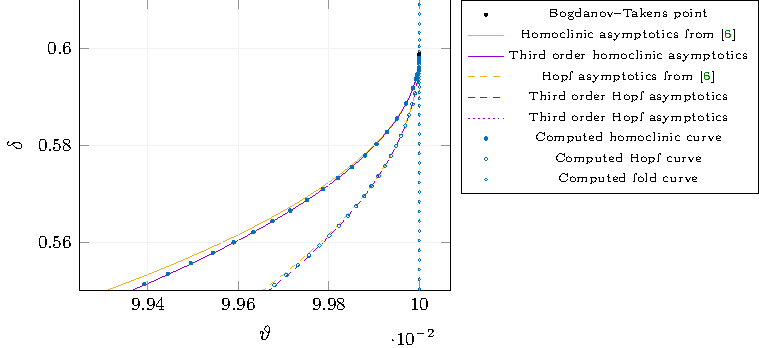
\includegraphics{\imagedir/DoubleAlleeEffectCompareParameters.pdf}
    \caption{Bifurcation diagram near the derived generic Bogdanov-Takens point in
        \cref{btdde:eq:double_alle_effect_rescaled} comparing computed codimension one
        using \DDEBIFTOOL with the asymptotics obtained in this paper and in \cite{Jiao2021}.}
    \label{btdde:fig:DoubleAlleeEffectCompareParameters}
\end{figure}
\begin{figure}[ht]
    \centering
    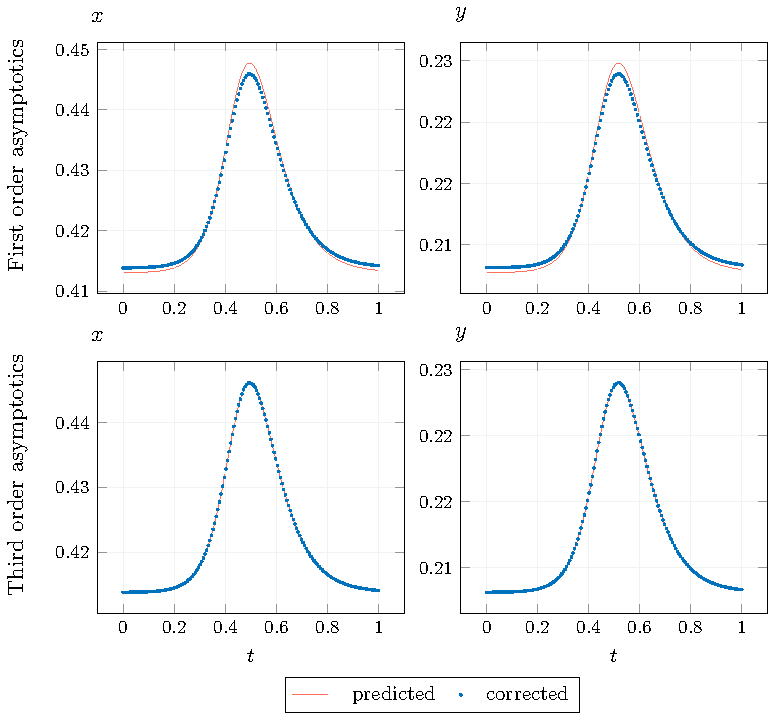
\includegraphics{\imagedir/DoubleAlleeEffectCompareProfiles.pdf}
    \caption{Comparison between the profiles of the first and third-order asymptotics from
    \cref{btdde:sec:generic_bt_homoclinic_asymptotics} with the Newton correct solutions near the generic
        Bogdanov--Takens bifurcation in \cref{btdde:eq:double_alle_effect_rescaled} with the
        perturbation parameter set to $\epsilon=0.3$.}
    \label{btdde:fig:DoubleAlleeEffectCompareProfiles}
\end{figure}
%
\begin{figure}[ht]
    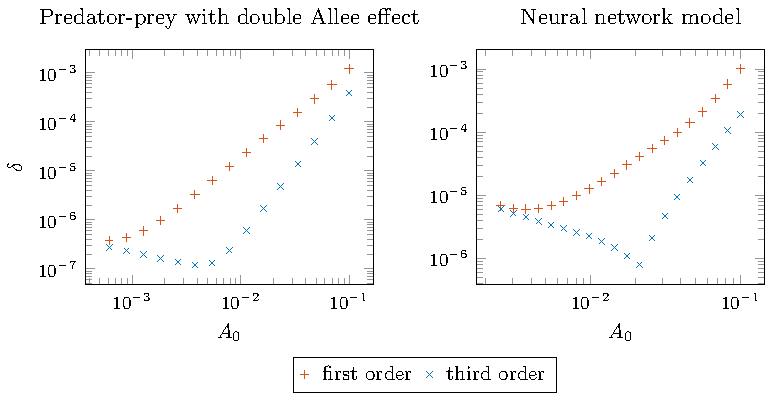
\includegraphics{\imagedir/convergencePlotsGeneric.pdf}
    \caption{On the abscissa is the approximation to the amplitude $A_0$ and on
        the ordinate the relative error $\delta$ between the constructed
        solution to the defining system
        \cite{connecting@2002} for the homoclinic orbit and the Newton
        corrected solution.}
    \label{btdde:fig:convergencePlotsGeneric}
\end{figure}
%
In \cite{Jiao2021} the following predator-prey model with double Allee effect and delay is considered
\begin{equation}
\label{btdde:eq:double_alle_effect}
\begin{cases}
    \dot x(t) = \dfrac{rx}{x+n_0}\left(1-\dfrac1 K\right)\left(x - m_0\right) - \dfrac{cxy}{x+\varrho y},\\
    \dot y(t) = -dy + \dfrac{c_1 x(t-\tau)y}{x(t-\tau) + \varrho y(t-\tau)}.
\end{cases}
\end{equation}
Here, the time delay $\tau \geq 0$ is introduced due to the fact that the
reproduction of predator after consuming the prey is not instantaneous, but is
mediated by some time lag required for gestation.
The variables and parameters occurring in \cref{btdde:eq:double_alle_effect}
have the following meaning:
\begin{itemize}
\item $x,y\colon \mathbb R \rightarrow \mathbb R$ denotes the prey and predator population density, respectively.
\item $r$ denotes the maximum prey population growth in absence of the Allee effect.
\item $K$ is the carrying capacity of the environment.
\item $m_0$ is the Allee threshold.
\item $n_0$ is the auxiliary parameter in order to quantify the strength of the Allee effect.
\item $c$ denotes the capturing rate of the predator.
\item $\varrho$ is the half capturing saturation constant.
\item $c_1$ is the conversion rate of prey into predators biomass.
\item $d$ is the per capita predator mortality rate.
\end{itemize}
Following \cite{Jiao2021} let $(x,y,t) = \left(K\bar x, \frac K \varrho \bar y, \frac{\bar t}r\right)$, and immediately 
dropping the bars again for readability, then \cref{btdde:eq:double_alle_effect} becomes
\begin{equation}
\label{btdde:eq:double_alle_effect_rescaled}
\begin{cases}
    \dot x(t) = x \left( \dfrac{(1-x)(x-\gamma)}{x+\vartheta} - \dfrac{\alpha y}{x+y} \right), \\
    \dot y(t) = \delta y \left( -1 + \dfrac{ m x(t-\tau) }{ x(t-\tau) + y(t-\tau) }\right),
\end{cases}
\end{equation}
where $\vartheta = \frac{n_0}K, \alpha=\frac c{r\varrho}, \gamma = \frac{m_0}K, \delta = \frac dr$ and $m=\frac{c_1}d$.
In \cite{Jiao2021} the phase-space is (although possible) unnecessarily
enlarged to include a parameter. The resulting extended system is used to
derive conditions for a Bogdanov--Takens bifurcation to occur and obtain the
normal form on the center manifold. In our opinion, one should only use the
extended system to prove the existence of a parameter-dependent center manifold,
from which it then follows that we can preform the normalization method as
described in \cref{btdde:sec:Center_manifold_reduction}. Thus, solving \cref{btdde:eq:double_alle_effect_rescaled}
for a double equilibrium with respect to $(x,y)$ and $\vartheta$ yields
\begin{equation}
    \begin{cases}
        x_0 = \dfrac{m+\alpha-m\alpha+m\gamma}{2m}, \\
        y_0 = (m-1)x_0, \\
        \vartheta_0 = \dfrac{(\alpha+m(1-\alpha+\gamma))^2 - 4m^2\gamma}{4(m-1)m\alpha},
    \end{cases}
\end{equation}
for $m\neq 1$. The parameters should of course be chosen such that $x$ and $y$
are non-negative. The characteristic matrix at
$(x,y,\vartheta)=(x_0,y_0,\vartheta_0)$ becomes
\[
\begingroup
\renewcommand*{\arraystretch}{2.5}
    \Delta(z) = \begin{pmatrix}
        z + \dfrac{1-m}{m^2}\alpha & \dfrac \alpha {m^2} \\
        -\dfrac{(m-1)^2\delta}m e^{-z\tau} & z + \dfrac{(m-1)\delta}m e^{-z\tau},
    \end{pmatrix}
\endgroup
\]
for $m\neq 0$. A simple calculation confirms indeed that $\det\Delta(0)=0$.
Furthermore, $\det\Delta'(0)=\frac{(m-1)(m\delta-\alpha)}{m^2}$ and
$\det\Delta''(0)=2 - \frac{2 (m-1) \delta\tau}{m}$. Thus, for
$(x,y,\vartheta,\delta)=(x_0,y_0,\vartheta_0,\delta_0)$, with $\delta_0 =
\frac\alpha m$, we have a double zero eigenvalue, provided that
$\det\Delta''(0) \neq 0$. To confirm their analytical findings in \cite{Jiao2021}
numerically, the parameters $\gamma=0.15,\alpha=0.9$ and $m=1.50298303$ are
fixed and $(\vartheta,\delta)$ are taken as unfolding parameters. For these
parameters, we indeed have that $\det\Delta''(0) \neq 0$. Calculating the normal
form coefficients $a$ and $b$ reveal that,
\[
a \approx 0.1479, \qquad b \approx 1.4457.
\]
Thus, the codimension two Bogdanov--Takens bifurcation is non-degenerate.
Furthermore, since the equilibrium $(x_0,y_0)$ depends on the unfolding
parameters, we are in the generic case. Using our implementation of the
homoclinic predictor \cref{btdde:sec:generic_bt_homoclinic_asymptotics} in
\DDEBIFTOOL we start the continuation of the homoclinic branch emanating from
the Bogdanov--Takens point.

In \cref{btdde:fig:DoubleAlleeEffectCompareParameters} we compare the parameters of
the computed homoclinic branch with our third-order parameter asymptotics and
the parameters for the homoclinic branch given in \cite{Jiao2021}. We observe
that although the derivation of the asymptotics for the parameters is
non-rigorous, it provides a good predictor. Nonetheless, our third-order
asymptotics for the parameter values provides clearly a better approximation to
the parameter values of the computed homoclinic branch.

Of course, most work lies in the derivation of the asymptotics for the
homoclinic solutions in phase-space itself, which is not available in
\cite{Jiao2021}. In  \cref{btdde:fig:DoubleAlleeEffectCompareProfiles} we compare the
first and third-order asymptotics for the profiles of the homoclinic solution.
Here we set the perturbation parameter to $\epsilon=0.3$ such that both
approximations converge, but we can visually observe a difference.

However, a numerical better way to compare the first and third-order
asymptotics for the homoclinic solution is through the use of a convergence
plots, similarly as in \cite{Bosschaert@Interplay}. In
\cref{btdde:fig:convergencePlotsGeneric} we clearly see an improvement of using the
third-order asymptotics over the first order asymptotics. We furthermore
observe the standard V-shaped graphs due to roundoff error.
\begin{figure}[ht]
    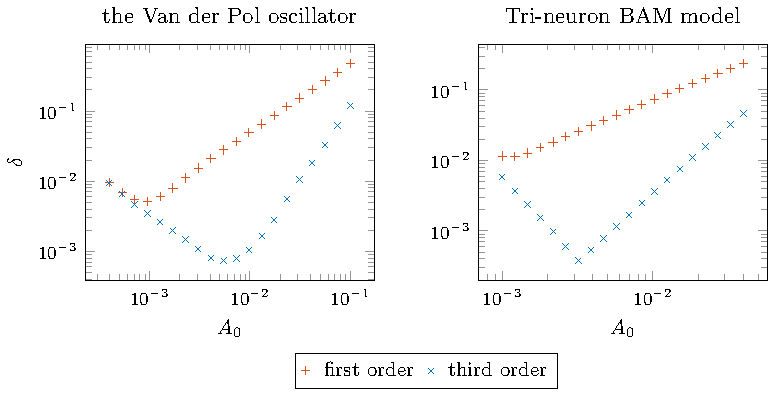
\includegraphics{\imagedir/convergencePlotsTranscritical.pdf}
    \caption{On the abscissa is the approximation to the amplitude $A_0$ and on
        the ordinate the relative error $\delta$ between the constructed solution
        to the defining system for the homoclinic orbit
        and the Newton corrected solution.}
    \label{btdde:fig:convergencePlotsTranscritical}
\end{figure}

\subsection{\ifthesis \phantom{ } \fi Generic Generic Bogdanov--Takens bifurcation in a neural network model}
In this example, we will consider the model 
\begin{equation}
\label{btdde:eq:neural_network}
\begin{cases}
\mu\dot{u}_1(t) = -u_1(t) + q_{11}\alpha(u_1(t\text{-}T))-q_{12}u_2(t\text{-}T) + e_1,\\
\mu\dot{u}_2(t) = -u_2(t) + q_{21}\alpha(u_1(t\text{-}T))-q_{22}u_2(t\text{-}T) + e_2,
\end{cases}
\end{equation}
which describes the dynamics of a neural network consisting of an
excitatory and inhibitory neurons \cite{giannakopoulos2001bifurcations}.
The variables and parameters occurring in \cref{btdde:eq:neural_network}
have the following neurophysiological meaning:
\begin{itemize}
\item $u_1,u_2:\mathbb{R}\rightarrow\mathbb{R}$ denote the total post-synaptic
potential of the excitatory and inhibitory neuron, respectively.
\item $\mu>0$ is a time constant characterizing the dynamical properties
of cell membrane.
\item $q_{ik}\geq0$ represents the strength of the connection line from
the $k$th neuron to the $i$th neuron.
\item $\alpha:\mathbb{R}\rightarrow\mathbb{R}$ is the transfer function
which describes the activity generation of the excitatory neuron as
a function of its total potential $u_1$. The function $\alpha$
is smooth, increasing and has a unique turning point at $u_1 = \theta$.
The transfer function corresponding to the inhibitory neuron is assumed
to be the identity.
\item $T\geq0$ is a time delay reflecting synaptic delay, axonal and dendritic
propagation time.
\item $e_1$ and $e_2$ are external stimuli acting on the excitatory
and inhibitory neuron, respectively.
\end{itemize}

Following \cite{giannakopoulos2001bifurcations} we consider the equation \cref{btdde:eq:neural_network} with
\begin{align*}
\alpha(u_1) & = \frac{1}{1 + e^{-4u_1}}-\frac{1}{2},\qquad q_{11} = 2.6,\qquad q_{21} = 1.0,\qquad q_{22} = 0.0,\\
\mu & = 1.0,\qquad T = 1.0,\qquad e_2 = 0.0,
\end{align*}
and $Q: = q_{12},\,E: = e_1$ as bifurcation parameters. Substituting
into \cref{btdde:eq:neural_network} yields
\begin{equation}
\label{btdde:eq:neural_network_subs}
\begin{cases}
\dot{u}_1(t) = -u_1(t) + 2.6\alpha(u_1(t - 1))-Qu_2(t - 1) + E,\\
\dot{u}_2(t) = -u_2(t) + \alpha(u_1(t - 1)).
\end{cases}
\end{equation}
Notice that for any steady-state we have the symmetry
$(u_1,u_2,E)\rightarrow(-u_1,-u_2,-E)$. It is easy to explicitly derive that the system has a double eigenvalue zero for
\begin{equation}
    \left\{
    \begin{aligned}
        u_1(t) &= \frac14 \log\left(\frac{8 - \sqrt{39}}5\right) \approx -0.2617, \\
        u_2(t) &= -\frac12 \sqrt{\frac{3}{13}} \approx -0.2402, \\
        Q &= \frac{13}{10}, \\
        E &= \frac{\sqrt{39} - 10\atanh \sqrt{\frac{3}{13}}}{20} \approx 0.0505.
    \end{aligned}\right.
\end{equation}

The dependence of $P_0$ on the parameters $(Q,E)$ yields a generic
Bogdanov--Takens bifurcation, see \cite{giannakopoulos2001bifurcations}. Notice
that the normal form reduction in \cite{giannakopoulos2001bifurcations} is
incorrect, which leads to the normal form for a transcritical Bogdanov--Takens
bifurcation.

\begin{figure}[ht]
    \centering
    \includetikzscaled{NeuralNetworkCompareParameters}
    \caption{Bifurcation diagram near the derived generic Bogdanov-Takens point in
        \cref{btdde:eq:neural_network_subs} comparing computed codimension one curves using
        \DDEBIFTOOL with the third-order homoclinic parameter asymptotics obtained
        in \cref{btdde:sec:generic_bt_homoclinic_asymptotics}.}
    \label{btdde:fig:NeuralNetworkCompareParameters}
\end{figure}

In \cref{btdde:fig:NeuralNetworkCompareParameters} we compared the computed
codimension one curves emanating from a generic Bogdanov--Takens point in
\cref{btdde:eq:neural_network_subs} using our implementation in \DDEBIFTOOL with the
third-order homoclinic parameter asymptotics obtained in
\cref{btdde:sec:generic_bt_homoclinic_asymptotics}. We see that the predicted and
computed curves are almost indistinguishable. Furthermore, in
\cref{btdde:fig:convergencePlotsGeneric} we see that using the third-order homoclinic
asymptotics over the first order is clearly superior.

\subsection{Transcritical Bogdanov--Takens bifurcation in the Van der Pol oscillator with delay feedback}
We consider the Van der Pol oscillator with delay feedback \cite{jiang2007bogdanov}
given by 
\begin{equation}
\ddot{x}(t) + \epsilon(x^2(t)-1)\dot{x}(t) + x(t) = \epsilon g(x(t-\tau))\label{btdde:eq:dde_vanderPol}
\end{equation}
where $\epsilon>0$ is a parameter, $\tau>0$ is a delay and $g:\mathbb{R}\rightarrow\mathbb{R}$
is a smooth function with $g(0) = 0$ and $g'(0)\neq0$. We rewrite
the Van der Pol equation \cref{btdde:eq:dde_vanderPol} as
\begin{equation}
\label{btdde:eq:vanderPolOscillator}
\begin{cases}
    \dot{x}_1 = x_2,\\
    \dot{x}_2 = \epsilon g(x_1(t-\tau))-\epsilon(x_1^2-1)x_2-x_1.
\end{cases}
\end{equation}
Rescaling time with $t\rightarrow\dfrac{t}{\tau}$ to normalize the
delay yields
\begin{equation}
\label{btdde:eq:vanderPolOscillatorRescaled}
\begin{cases}
\dot{x}_1 = \tau x_2,\\
\dot{x}_2 = \tau\left(\epsilon g(x_1(t-1))-\epsilon(x_1^2-1)x_2-x_1\right).
\end{cases}
\end{equation}
In this allows is to treat $\tau$ as a bifurcation parameter.

Following \cite{jiang2007bogdanov}, we consider \cref{btdde:eq:dde_vanderPol} with
\[
g(x) = \frac{e^x-1}{c_1e^x + c_2},
\]
where $c_1 = \dfrac{1}{4}$ and $c_2 = \dfrac{1}{2}$. Then the trivial
equilibrium undergoes a transcritical Bogdanov--Takens bifurcation at parameter
values $(\epsilon,\tau) = (0.75,0.75)$, \cite{jiang2007bogdanov} and the
supplement. 
%
\begin{figure}[ht]
    \centering
    \includetikzscaled{vanderPolOscillatorCompareParameters}
    \caption{Bifurcation diagram near the derived generic Bogdanov-Takens point in
        \cref{btdde:eq:vanderPolOscillatorRescaled} comparing computed codimension one curves using
        \DDEBIFTOOL with the third-order homoclinic parameter asymptotics obtained
        in \cref{btdde:sec:transcritical_bt_homoclinic_asymptotics}.}
    \label{btdde:fig:vanderPolOscillatorCompareParameters}
\end{figure}

In \cref{btdde:fig:vanderPolOscillatorCompareParameters} we compared the computed
codimension one curves emanating from a transcritical Bogdanov--Takens point in
\cref{btdde:eq:vanderPolOscillatorRescaled} using our implementation in \DDEBIFTOOL
with the third-order homoclinic parameter asymptotics obtained in
\cref{btdde:sec:transcritical_bt_homoclinic_asymptotics}. We see that the predicted
and computed curves are almost indistinguishable. Furthermore, in
\cref{btdde:fig:convergencePlotsTranscritical} we see that using the third-order
homoclinic asymptotics over the first order is clearly superior.

\subsection{Transcritical Bogdanov--Takens bifurcation in a Tri-neuron BAM neural network model}
\label{btdde:sec:Tri-neuron-BAM-neural}

We consider a three-component system of a Tri-neuron BAM (bidirectional
associative memory) neural network model with multiple delays \cite{dong2013bogdanov}.
The architecture of this BAM model is illustrated in \cref{btdde:fig:BAM_architecture_graph}. 

\begin{figure}
\centering
\includetikzscaled[0.75]{BAM_architecture_graph}
\caption{The graph of architecture for model \cref{btdde:eq:tri_neuron_BAM}.}
\label{btdde:fig:BAM_architecture_graph}
\end{figure}

\begin{figure}[ht]
\centering
\includetikzscaled{triNeuronBAMNeuralNetworkModelCompareParameters}
\caption{
Bifurcation diagram near the transcritical Bogdanov--Takens bifurcation and
a generic Bogdanov--Takens in \cref{btdde:eq:tri_neuron_BAM-u} comparing computed
codimension one using \DDEBIFTOOL with the asymptotics obtained in this
paper.}
\label{btdde:fig:triNeuronBAMNeuralNetworkModelCompareParameters}
\end{figure}

In this model, there is only one neuron with the activation function
$f_{1}$ on the $I$-layer and there are two neurons with respective
activation functions $f_{2}$ and $f_{3}$ on the $J$-layer. It is assumed 
that the time delay from the $I$-layer to the $J$-layer is $\tau_{1}$,
while the time delay from the $J$-layer to the $I$-layer is $\tau_{2}$.
Then the network can be described by the following delay differential equation:
\begin{equation}
\label{btdde:eq:tri_neuron_BAM}
\begin{cases}
\dot{x}_{1}(t) & =-\mu_{1}x_{1}(t)+c_{21}f_{1}(x_{2}(t-\tau_{2}))+c_{31}f_{1}(x_{3}(t-\tau_{2})),\\
\dot{x}_{2}(t) & =-\mu_{2}x_{2}(t)+c_{12}f_{2}(x_{1}(t-\tau_{1})),\\
\dot{x}_{3}(t) & =-\mu_{3}x_{3}(t)+c_{13}f_{3}(x_{1}(t-\tau_{1})).
\end{cases}
\end{equation}
Here
\begin{itemize}
\item $x_{i}(t)\,(i=1,2,3)$ denote the state of the neuron at time $t$;
\item $\mu_{i}(i=1,2,3)$ describe the attenuation rate of internal neurons
processing on the $I$-layer and the $J$-layer and $\mu_{i}>0$;
\item the real constants $c_{i1}$and $c_{1i}\,(2,3)$ denote the neurons
in two layers: the $I$-layer and the $J$-layer.
\end{itemize}
Letting $u_{1}(t)=x_{1}(t-\tau_{1}),u_{2}(t)=x_{2}(t),u_{3}(t)=x_{3}(t)$
and $\tau=\tau_{1}+\tau_{2}$, then system \cref{btdde:eq:tri_neuron_BAM}
is equivalent to the following system:

\begin{equation}
\label{btdde:eq:tri_neuron_BAM-u}
\begin{cases}
\dot{u}_{1}(t) & =-\mu_{1}u_{1}(t)+c_{21}f_{1}(u_{2}(t-\tau))+c_{31}f_{1}(u_{3}(t-\tau)),\\
\dot{u}_{2}(t) & =-\mu_{2}u_{2}(t)+c_{12}f_{2}(u_{1}(t)),\\
\dot{u}_{3}(t) & =-\mu_{3}u_{3}(t)+c_{13}f_{3}(u_{1}(t)).
\end{cases}
\end{equation}

In \cite{dong2013bogdanov} conditions form \cref{btdde:eq:tri_neuron_BAM-u} are derived
for the origin to have a double zero eigenvalue, while all other eigenvalues
have negative real parts. Since the provided expression didn't give the correct results,
we corrected the given expression form \cite{dong2013bogdanov}.
We postpone the proof of the next two lemma's to the
\ifthesis{\cref{chapter:BT_DDE_supplement}
}\else{\hyperref[mysupplement]{online Supplement} }\fi. 

\begin{lemma}
\label{btdde:lem:BAM_double_eigenvalue}
Assume that $f_{i}(0)=0\,(i=1,2,3)$,
$f_{i}'(0)\neq0\,(i=1,2,3)$ and $\mu_{2}\neq\mu_{3}$, then the steady-state
$(u_{1},u_{2},u_{3})=(0,0,0)$ has a double zero eigenvalue at 
\begin{align*}
c_{21} & =c_{21}^{0}=\frac{\mu_{2}^{2}\left(\mu_{1}\left(\mu_{3}\tau+1\right)+\mu_{3}\right)}{c_{12}\left(\mu_{2}-\mu_{3}\right)f_{1}'(0)f_{2}'(0)},\\
c_{31} & =c_{31}^{0}=\frac{\mu_{3}^{2}\left(\mu_{1}\left(\mu_{2}\tau+1\right)+\mu_{2}\right)}{c_{13}\left(\mu_{3}-\mu_{2}\right)f_{1}'(0)f_{3}'(0)}.
\end{align*}
\end{lemma}

\begin{lemma}
\label{btdde:lemma:triNeuralBAMNetworkModelEigenvalues}
\textup{Correction to \cite[Lemma 3]{dong2013bogdanov}}
Let $(c_{21},c_{31})=(c_{21}^{0},c_{31}^{0})$,
\begin{equation}
    \label{btdde:sm:eq:omega_0} 
    \omega_0 = \frac{\sqrt{-\mu_1^2 - \mu_2^2 - \mu_3^2 + \sqrt{\zeta_0}}}{\sqrt{2}}
\end{equation}
and $0<\tau<\tau_{0}$, where $\tau_0$ is the minimum positive solution to the nonlinear equation
\begin{equation}
    \label{btdde:sm:eq:tan} 
    \tan (\tau \omega_0) = \frac{b_0\zeta_1 - a_0\zeta_2}{a_0\zeta_1 + b_0\zeta_2},
\end{equation}
with
\begin{align*}
a_0 &= -\mu_1\mu_2\mu_3, \\ 
b_0 &= -\omega_0(\mu_2\mu_3 + \mu_1(\mu_2 + \mu_3 + \mu_2\mu_3\tau)), \\
\zeta_0 &= \mu_1^4 + (\mu_2^2 + \mu_3^2)^2 + 8\mu_1\mu_2\mu_3(\mu_2 + \mu_3 + \mu_2\mu_3\tau) + \\
        &\qquad 2\mu_1^2(\mu_3^2 + 4\mu_2\mu_3(1 + \mu_3\tau) + \mu_2^2(1 + 2\mu_3\tau(2 + \mu_3\tau))), \\
\zeta_1 &= \mu_1\mu_2\mu_3 - (\mu_1 + \mu_2 + \mu_3)\omega_0^2, \\
\zeta_2 &= \mu_2\mu_3\omega_0 + \mu_1(\mu_2 + \mu_3)\omega_0 - \omega_0^3.
\end{align*}
Then the center manifold near the Bogdanov--Takens point is locally attractive.
\end{lemma}

For the numerical verification we consider, as in the simulations in
\cite[Example 1]{dong2013bogdanov}, the system \cref{btdde:eq:tri_neuron_BAM-u} with
the activation functions
\[
f_{1}(x)=\tanh(x)+0.1x^{2},\quad f_{2}(x)=f_{3}(x)=\tanh(x),
\]
and parameters values
\[
\mu_{1}=0.1,\mu_{2}=0.3,\mu_{3}=0.2,c_{12}=c_{13}=1,\tau=5.
\]
Then from \cref{btdde:lem:BAM_double_eigenvalue} we obtain two critical
values 
\[
(c_{21}^{0},c_{31}^{0})=(0.36,-0.22),
\]
at which there is a transcritical Bogdanov--Takens point. Furthermore, since
$\tau < \tau_0 \approx 5.4320$ the center manifold is attractive. In fact, we
will show in the
\ifthesis{\cref{chapter:BT_DDE_supplement} }\else{\hyperref[mysupplement]{online
Supplement} }\fi that the center manifold is attractive for
$0<\tau<13.2309348879375$. We write the system \cref{btdde:eq:tri_neuron_BAM-u}
as
\begin{equation}
\label{btdde:eq:tri_neuron_BAM-u-1}
\begin{cases}
\dot{u}_{1}(t) & =-\mu_{1}u_{1}(t)+\left(c_{21}^{0}+\alpha_{1}\right)f_{1}(u_{2}(t-\tau))+\left(c_{31}^{0}+\alpha_{2}\right)f_{1}(u_{3}(t-\tau)),\\
\dot{u}_{2}(t) & =-\mu_{2}u_{2}(t)+c_{12}f_{2}(u_{1}(t)),\\
\dot{u}_{3}(t) & =-\mu_{3}u_{3}(t)+c_{13}f_{3}(u_{1}(t)),
\end{cases}
\end{equation}
where $(\alpha_{1},\alpha_{2})$ are the new parameter values such
that at $(\alpha_{1},\alpha_{2})=(0,0)$ we have a Bogdanov-Takens
bifurcation. The critical normal form coefficients 
\[
(a,b)\approx(0.0012,-0.0135),
\]
indicate stable cycles. In
\cref{btdde:fig:triNeuronBAMNeuralNetworkModelCompareParameters} we have plotted the
local unfolding of the transcritical Bogdanov-Takens bifurcation using our
implementation in DDE-BifTool to start the continuation of the transcritical,
Hopf, and homoclinic codimension one bifurcation curves. Furthermore, using the
ability to detect codimension two bifurcation points while continuing Hopf
points, we discovered another Bogdanov--Takens point. From the transversality
conditions, we see the secondary Bogdanov--Takens point is of the generic case.
Thus, we can start continuation of the homoclinic orbits emanating from this
point as well. We see that the numerically continued homoclinic curves in the
upper half plane only exists in a very small parameter region. Without our
predictor this homoclinic curve would be extremely difficult to locate. Lastly,
in \cref{btdde:fig:convergencePlotsTranscritical} compared the first and third-order
homoclinic asymptotics. Here we again see expected improvement of using the
third-order homoclinic asymptotics. We refer to the
\ifthesis{\cref{chapter:BT_DDE_supplement}
}\else{\hyperref[mysupplement]{online Supplement} }\fi to see the beautiful
homoclinic orbits along the homoclinic curve in the lower half plane, and for
an overall more detailed treatment of this example. In fact, we will show that
the transcritical Bogdanov--Takens and generic Bogdanov--Takens points are
connected, not only by a Hopf curve, but also through a homoclinic curve. 

\section{Concluding remarks}
We have provided explicit formulas needed to initialize the codimension one
equilibrium and homoclinic bifurcations emanating from the transcritical and
generalized codimension two Bogdanov--Takens bifurcation point is classical
DDEs. Applications to four different models are given, confirming the
correctness of the derivation for the time-reparametrization
parameter-dependent
center manifold transformation and the asymptotics.

By extending the normalization technique to include a time-reparametrization we
are allowed to use orbital normal forms, instead of only smooth normal forms.
One benefit of this approach is the reusability of the codimension one curves
emanating from the universal unfolding of the Bogdanov--Takens codimension two
bifurcation. Indeed, by a simple transformation \cref{btdde:eq:blowup} we obtain the
homoclinic asymptotics for the transcritical Bogdanov--Takens bifurcation.

It this paper we have restricted to the class of classical DDEs, and for the
applications to the class of discrete DDEs. However, the proof in
\cite{Switching2019} of the existence of a smooth parameter-dependent center
manifold is given in the general context of perturbation theory for dual
semigroups (sun-star calculus). Therefore, the applicability of this result
extends beyond classical DDEs, For example, in \cite{VanGils2013} and
\cite{Dijkstra2015} the technique was used to calculate the critical normal
form coefficients for Hopf and Hopf-Hopf bifurcations occurring in neural field
models with propagation delays. For these models, sun-reflexivity is lost, which
is typical for delay equations in abstract spaces or with infinite delay.
However, it is often possible to overcome this functional analytic
complication, so dual perturbation theory can still be employed successfully
\cite{Diekmann2008,Diekmann2012blending,VanGils2013,Janssens2019}. It follows
that the derived coefficients in
\cref{btdde:sec:parameter-dependent-center-manifold-reduction} are valid in these
settings as well.

Similarly, in \cite{Sieber@2017} it is demonstrated that formally the
normalization method still works for DDEs with state-dependent delays.
However, for our formulas to work in this situation, one first needs
to implement the continuation of homoclinic orbits for state-dependent
DDEs. Of course, the asymptotics are still useful to see where     the 
homoclinic orbit should be located. Furthermore, the asymptotics
can be used to numerically approximate the homoclinic solutions by periodic
orbits with a large return time.

Returning to the setting of classical DDEs, the most obvious next challenge is
to derive normal forms for bifurcations of periodic orbits by generalizing
\cite{Kuznetsov2005,DeWitte2013,DeWitte2014}. The resulting formulas can then
be implemented in \DDEBIFTOOL to facilitate numerical bifurcation analysis of
periodic orbits in supported types of classical DDEs.
